\documentclass[twoside]{book}

% Packages required by doxygen
\usepackage{fixltx2e}
\usepackage{calc}
\usepackage{doxygen}
\usepackage[export]{adjustbox} % also loads graphicx
\usepackage{graphicx}
\usepackage[utf8]{inputenc}
\usepackage{makeidx}
\usepackage{multicol}
\usepackage{multirow}
\PassOptionsToPackage{warn}{textcomp}
\usepackage{textcomp}
\usepackage[nointegrals]{wasysym}
\usepackage[table]{xcolor}

% Font selection
\usepackage[T1]{fontenc}
\usepackage[scaled=.90]{helvet}
\usepackage{courier}
\usepackage{amssymb}
\usepackage{sectsty}
\renewcommand{\familydefault}{\sfdefault}
\allsectionsfont{%
  \fontseries{bc}\selectfont%
  \color{darkgray}%
}
\renewcommand{\DoxyLabelFont}{%
  \fontseries{bc}\selectfont%
  \color{darkgray}%
}
\newcommand{\+}{\discretionary{\mbox{\scriptsize$\hookleftarrow$}}{}{}}

% Page & text layout
\usepackage{geometry}
\geometry{%
  a4paper,%
  top=2.5cm,%
  bottom=2.5cm,%
  left=2.5cm,%
  right=2.5cm%
}
\tolerance=750
\hfuzz=15pt
\hbadness=750
\setlength{\emergencystretch}{15pt}
\setlength{\parindent}{0cm}
\setlength{\parskip}{3ex plus 2ex minus 2ex}
\makeatletter
\renewcommand{\paragraph}{%
  \@startsection{paragraph}{4}{0ex}{-1.0ex}{1.0ex}{%
    \normalfont\normalsize\bfseries\SS@parafont%
  }%
}
\renewcommand{\subparagraph}{%
  \@startsection{subparagraph}{5}{0ex}{-1.0ex}{1.0ex}{%
    \normalfont\normalsize\bfseries\SS@subparafont%
  }%
}
\makeatother

% Headers & footers
\usepackage{fancyhdr}
\pagestyle{fancyplain}
\fancyhead[LE]{\fancyplain{}{\bfseries\thepage}}
\fancyhead[CE]{\fancyplain{}{}}
\fancyhead[RE]{\fancyplain{}{\bfseries\leftmark}}
\fancyhead[LO]{\fancyplain{}{\bfseries\rightmark}}
\fancyhead[CO]{\fancyplain{}{}}
\fancyhead[RO]{\fancyplain{}{\bfseries\thepage}}
\fancyfoot[LE]{\fancyplain{}{}}
\fancyfoot[CE]{\fancyplain{}{}}
\fancyfoot[RE]{\fancyplain{}{\bfseries\scriptsize Generated by Doxygen }}
\fancyfoot[LO]{\fancyplain{}{\bfseries\scriptsize Generated by Doxygen }}
\fancyfoot[CO]{\fancyplain{}{}}
\fancyfoot[RO]{\fancyplain{}{}}
\renewcommand{\footrulewidth}{0.4pt}
\renewcommand{\chaptermark}[1]{%
  \markboth{#1}{}%
}
\renewcommand{\sectionmark}[1]{%
  \markright{\thesection\ #1}%
}

% Indices & bibliography
\usepackage{natbib}
\usepackage[titles]{tocloft}
\setcounter{tocdepth}{3}
\setcounter{secnumdepth}{5}
\makeindex

% Hyperlinks (required, but should be loaded last)
\usepackage{ifpdf}
\ifpdf
  \usepackage[pdftex,pagebackref=true]{hyperref}
\else
  \usepackage[ps2pdf,pagebackref=true]{hyperref}
\fi
\hypersetup{%
  colorlinks=true,%
  linkcolor=blue,%
  citecolor=blue,%
  unicode%
}

% Custom commands
\newcommand{\clearemptydoublepage}{%
  \newpage{\pagestyle{empty}\cleardoublepage}%
}

\usepackage{caption}
\captionsetup{labelsep=space,justification=centering,font={bf},singlelinecheck=off,skip=4pt,position=top}

%===== C O N T E N T S =====

\begin{document}

% Titlepage & ToC
\hypersetup{pageanchor=false,
             bookmarksnumbered=true,
             pdfencoding=unicode
            }
\pagenumbering{alph}
\begin{titlepage}
\vspace*{7cm}
\begin{center}%
{\Large color\+\_\+flood \\[1ex]\large 1.\+0 }\\
\vspace*{1cm}
{\large Generated by Doxygen 1.8.13}\\
\end{center}
\end{titlepage}
\clearemptydoublepage
\pagenumbering{roman}
\tableofcontents
\clearemptydoublepage
\pagenumbering{arabic}
\hypersetup{pageanchor=true}

%--- Begin generated contents ---
\chapter{Data Structure Index}
\section{Data Structures}
Here are the data structures with brief descriptions\+:\begin{DoxyCompactList}
\item\contentsline{section}{\hyperlink{structbutton}{button} }{\pageref{structbutton}}{}
\item\contentsline{section}{\hyperlink{structmenu}{menu} }{\pageref{structmenu}}{}
\item\contentsline{section}{\hyperlink{structnode}{node} }{\pageref{structnode}}{}
\item\contentsline{section}{\hyperlink{structsdl_board}{sdl\+Board} }{\pageref{structsdl_board}}{}
\item\contentsline{section}{\hyperlink{structsdl_preview}{sdl\+Preview} }{\pageref{structsdl_preview}}{}
\item\contentsline{section}{\hyperlink{structsettings_screen}{settings\+Screen} }{\pageref{structsettings_screen}}{}
\item\contentsline{section}{\hyperlink{structt__game}{t\+\_\+game} \\*Structure de la partie }{\pageref{structt__game}}{}
\item\contentsline{section}{\hyperlink{structt__grid}{t\+\_\+grid} \\*Structure d\textquotesingle{}une grille }{\pageref{structt__grid}}{}
\item\contentsline{section}{\hyperlink{structt___r_g_b}{t\+\_\+\+R\+GB} \\*Structure d\textquotesingle{}une couleur en utilisant le code rgb }{\pageref{structt___r_g_b}}{}
\item\contentsline{section}{\hyperlink{structtextbox}{textbox} }{\pageref{structtextbox}}{}
\item\contentsline{section}{\hyperlink{structtexture}{texture} }{\pageref{structtexture}}{}
\end{DoxyCompactList}

\chapter{File Index}
\section{File List}
Here is a list of all documented files with brief descriptions\+:\begin{DoxyCompactList}
\item\contentsline{section}{src/game/\hyperlink{game_8c}{game.\+c} \\*Gestion du jeu pendant une partie }{\pageref{game_8c}}{}
\item\contentsline{section}{src/game/{\bfseries game.\+h} }{\pageref{game_8h}}{}
\item\contentsline{section}{src/game/\hyperlink{grid_8c}{grid.\+c} \\*Gestion de la grille de jeu }{\pageref{grid_8c}}{}
\item\contentsline{section}{src/game/{\bfseries grid.\+h} }{\pageref{grid_8h}}{}
\item\contentsline{section}{src/game/\hyperlink{rgb_8c}{rgb.\+c} \\*Gestion des couleurs }{\pageref{rgb_8c}}{}
\item\contentsline{section}{src/game/{\bfseries rgb.\+h} }{\pageref{rgb_8h}}{}
\item\contentsline{section}{src/sdl/{\bfseries button\+\_\+wrapper.\+h} }{\pageref{button__wrapper_8h}}{}
\item\contentsline{section}{src/sdl/{\bfseries game\+\_\+board\+\_\+rendering.\+h} }{\pageref{game__board__rendering_8h}}{}
\item\contentsline{section}{src/sdl/{\bfseries game\+\_\+load\+\_\+rendering.\+h} }{\pageref{game__load__rendering_8h}}{}
\item\contentsline{section}{src/sdl/{\bfseries game\+\_\+menu\+\_\+rendering.\+h} }{\pageref{game__menu__rendering_8h}}{}
\item\contentsline{section}{src/sdl/{\bfseries game\+\_\+settings\+\_\+rendering.\+h} }{\pageref{game__settings__rendering_8h}}{}
\item\contentsline{section}{src/sdl/{\bfseries game\+\_\+states.\+h} }{\pageref{game__states_8h}}{}
\item\contentsline{section}{src/sdl/{\bfseries sdl\+\_\+utils.\+h} }{\pageref{sdl__utils_8h}}{}
\item\contentsline{section}{src/sdl/{\bfseries textbox\+\_\+wrapper.\+h} }{\pageref{textbox__wrapper_8h}}{}
\item\contentsline{section}{src/sdl/{\bfseries texture\+\_\+wrapper.\+h} }{\pageref{texture__wrapper_8h}}{}
\item\contentsline{section}{src/solver/\hyperlink{solver_8c}{solver.\+c} \\*Gestion du solveur }{\pageref{solver_8c}}{}
\item\contentsline{section}{src/solver/{\bfseries solver.\+h} }{\pageref{solver_8h}}{}
\item\contentsline{section}{src/solver/{\bfseries stack.\+h} }{\pageref{stack_8h}}{}
\end{DoxyCompactList}

\chapter{Data Structure Documentation}
\hypertarget{structbutton}{}\section{button Struct Reference}
\label{structbutton}\index{button@{button}}


Collaboration diagram for button\+:
\nopagebreak
\begin{figure}[H]
\begin{center}
\leavevmode
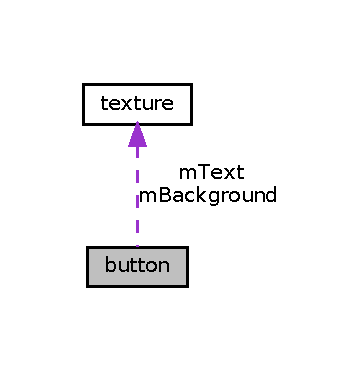
\includegraphics[width=174pt]{structbutton__coll__graph}
\end{center}
\end{figure}
\subsection*{Data Fields}
\begin{DoxyCompactItemize}
\item 
\mbox{\Hypertarget{structbutton_a565fe26ba3de4ef01d9d6a4b6b6725d2}\label{structbutton_a565fe26ba3de4ef01d9d6a4b6b6725d2}} 
S\+D\+L\+\_\+\+Point {\bfseries m\+Position}
\item 
\mbox{\Hypertarget{structbutton_a7eb136dcc643483eb579ed938c3cee33}\label{structbutton_a7eb136dcc643483eb579ed938c3cee33}} 
\hyperlink{structtexture}{L\+Texture} $\ast$ {\bfseries m\+Background}
\item 
\mbox{\Hypertarget{structbutton_a411a3221c211bc7bc0a98ad71b16d288}\label{structbutton_a411a3221c211bc7bc0a98ad71b16d288}} 
\hyperlink{structtexture}{L\+Texture} $\ast$ {\bfseries m\+Text}
\item 
\mbox{\Hypertarget{structbutton_aaf55b59bca0d347c78a27dff0a9b201a}\label{structbutton_aaf55b59bca0d347c78a27dff0a9b201a}} 
enum L\+Button\+State {\bfseries s}
\item 
\mbox{\Hypertarget{structbutton_a24b7101872d741490b84d97fcfb6ea48}\label{structbutton_a24b7101872d741490b84d97fcfb6ea48}} 
void($\ast$ {\bfseries trigger\+Ptr} )(int $\ast$)
\end{DoxyCompactItemize}


The documentation for this struct was generated from the following file\+:\begin{DoxyCompactItemize}
\item 
src/sdl/button\+\_\+wrapper.\+h\end{DoxyCompactItemize}

\hypertarget{structmenu}{}\section{menu Struct Reference}
\label{structmenu}\index{menu@{menu}}


Collaboration diagram for menu\+:
\nopagebreak
\begin{figure}[H]
\begin{center}
\leavevmode
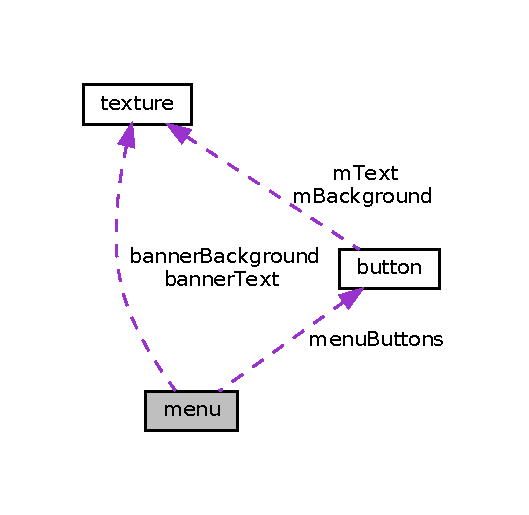
\includegraphics[width=254pt]{structmenu__coll__graph}
\end{center}
\end{figure}
\subsection*{Data Fields}
\begin{DoxyCompactItemize}
\item 
\mbox{\Hypertarget{structmenu_aec81a913a2bdf7db9fa55631ac232cbd}\label{structmenu_aec81a913a2bdf7db9fa55631ac232cbd}} 
T\+T\+F\+\_\+\+Font $\ast$ {\bfseries menu\+Font}
\item 
\mbox{\Hypertarget{structmenu_a48e5d82d2c83eb5f30f0b5329a15f103}\label{structmenu_a48e5d82d2c83eb5f30f0b5329a15f103}} 
size\+\_\+t {\bfseries font\+Size}
\item 
\mbox{\Hypertarget{structmenu_aa3c91e91465b65a7dc5a3245b6e105f7}\label{structmenu_aa3c91e91465b65a7dc5a3245b6e105f7}} 
\hyperlink{structtexture}{L\+Texture} $\ast$ {\bfseries banner\+Text}
\item 
\mbox{\Hypertarget{structmenu_aa8e15e8629ba7f2cdab66418f4e8647b}\label{structmenu_aa8e15e8629ba7f2cdab66418f4e8647b}} 
\hyperlink{structtexture}{L\+Texture} $\ast$ {\bfseries banner\+Background}
\item 
\mbox{\Hypertarget{structmenu_aaa6a726c45ebf13e6ce59e69a82aca4a}\label{structmenu_aaa6a726c45ebf13e6ce59e69a82aca4a}} 
\hyperlink{structbutton}{L\+Button} $\ast$ {\bfseries menu\+Buttons} \mbox{[}M\+E\+N\+U\+\_\+\+B\+U\+T\+T\+O\+N\+S\+\_\+\+C\+O\+U\+NT\mbox{]}
\item 
\mbox{\Hypertarget{structmenu_a04da60f12d502931bdcc034cad86347f}\label{structmenu_a04da60f12d502931bdcc034cad86347f}} 
S\+D\+L\+\_\+\+Window $\ast$$\ast$ {\bfseries g\+Window}
\item 
\mbox{\Hypertarget{structmenu_ad916adf6a3c707eda83ceefbdee69a26}\label{structmenu_ad916adf6a3c707eda83ceefbdee69a26}} 
S\+D\+L\+\_\+\+Renderer $\ast$$\ast$ {\bfseries g\+Renderer}
\end{DoxyCompactItemize}


The documentation for this struct was generated from the following file\+:\begin{DoxyCompactItemize}
\item 
src/sdl/game\+\_\+menu\+\_\+rendering.\+h\end{DoxyCompactItemize}

\hypertarget{structnode}{}\section{node Struct Reference}
\label{structnode}\index{node@{node}}


Collaboration diagram for node\+:
\nopagebreak
\begin{figure}[H]
\begin{center}
\leavevmode
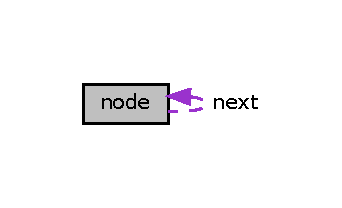
\includegraphics[width=164pt]{structnode__coll__graph}
\end{center}
\end{figure}
\subsection*{Data Fields}
\begin{DoxyCompactItemize}
\item 
\mbox{\Hypertarget{structnode_a9eab91667db4d35c7231dcddf7b89a76}\label{structnode_a9eab91667db4d35c7231dcddf7b89a76}} 
int {\bfseries data}
\item 
\mbox{\Hypertarget{structnode_a0dc1b6470487aa86d9936e3cab8b95be}\label{structnode_a0dc1b6470487aa86d9936e3cab8b95be}} 
struct \hyperlink{structnode}{node} $\ast$ {\bfseries next}
\end{DoxyCompactItemize}


The documentation for this struct was generated from the following file\+:\begin{DoxyCompactItemize}
\item 
src/solver/stack.\+h\end{DoxyCompactItemize}

\hypertarget{structsdl_board}{}\section{sdl\+Board Struct Reference}
\label{structsdl_board}\index{sdl\+Board@{sdl\+Board}}


Collaboration diagram for sdl\+Board\+:
\nopagebreak
\begin{figure}[H]
\begin{center}
\leavevmode
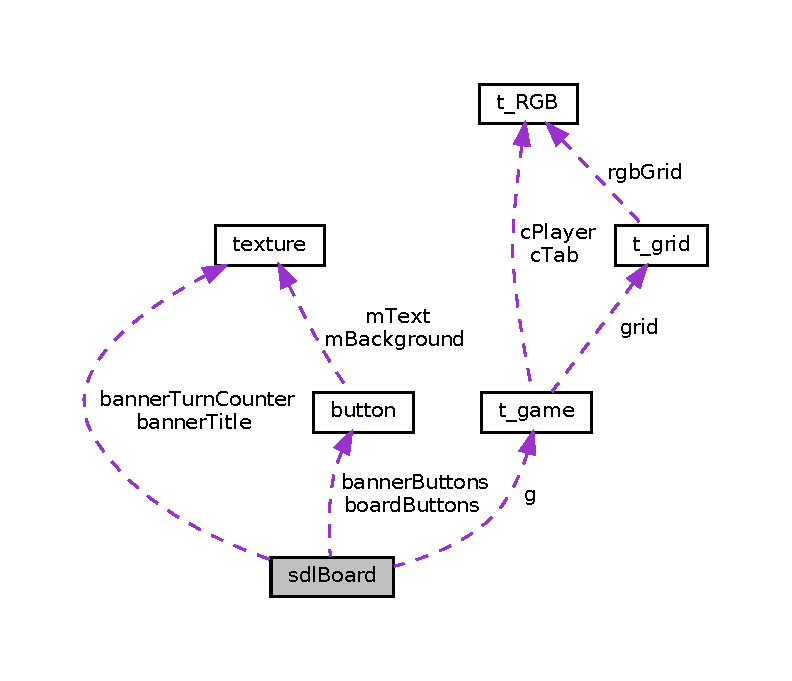
\includegraphics[width=350pt]{structsdl_board__coll__graph}
\end{center}
\end{figure}
\subsection*{Data Fields}
\begin{DoxyCompactItemize}
\item 
\mbox{\Hypertarget{structsdl_board_a04da60f12d502931bdcc034cad86347f}\label{structsdl_board_a04da60f12d502931bdcc034cad86347f}} 
S\+D\+L\+\_\+\+Window $\ast$$\ast$ {\bfseries g\+Window}
\item 
\mbox{\Hypertarget{structsdl_board_ad916adf6a3c707eda83ceefbdee69a26}\label{structsdl_board_ad916adf6a3c707eda83ceefbdee69a26}} 
S\+D\+L\+\_\+\+Renderer $\ast$$\ast$ {\bfseries g\+Renderer}
\item 
\mbox{\Hypertarget{structsdl_board_a108a55905975a9bc5f2486e3284fc86e}\label{structsdl_board_a108a55905975a9bc5f2486e3284fc86e}} 
T\+T\+F\+\_\+\+Font $\ast$ {\bfseries banner\+Font}
\item 
\mbox{\Hypertarget{structsdl_board_a3f3b791c64b074b7d315a41416fd452d}\label{structsdl_board_a3f3b791c64b074b7d315a41416fd452d}} 
\hyperlink{structt__game}{game} $\ast$ {\bfseries g}
\item 
\mbox{\Hypertarget{structsdl_board_a69bf27f2296ddb5e24d78f17832a16ec}\label{structsdl_board_a69bf27f2296ddb5e24d78f17832a16ec}} 
int {\bfseries max\+Turns}
\item 
\mbox{\Hypertarget{structsdl_board_a0e572169338230e30d01a3b1af9324a1}\label{structsdl_board_a0e572169338230e30d01a3b1af9324a1}} 
\hyperlink{structtexture}{L\+Texture} $\ast$ {\bfseries banner\+Title}
\item 
\mbox{\Hypertarget{structsdl_board_aa575bc57abd27271283775a414c5721b}\label{structsdl_board_aa575bc57abd27271283775a414c5721b}} 
\hyperlink{structtexture}{L\+Texture} $\ast$ {\bfseries banner\+Turn\+Counter}
\item 
\mbox{\Hypertarget{structsdl_board_a898a14b8dbc4ff8f956752cbd5df0aab}\label{structsdl_board_a898a14b8dbc4ff8f956752cbd5df0aab}} 
\hyperlink{structbutton}{L\+Button} $\ast$ {\bfseries banner\+Buttons} \mbox{[}2\mbox{]}
\item 
\mbox{\Hypertarget{structsdl_board_ace03d870a8c8c0b9a2219cfbd2d5ffbc}\label{structsdl_board_ace03d870a8c8c0b9a2219cfbd2d5ffbc}} 
\hyperlink{structbutton}{L\+Button} $\ast$$\ast$ {\bfseries board\+Buttons}
\item 
\mbox{\Hypertarget{structsdl_board_a326ac0832310ae96cbae0f489eedac92}\label{structsdl_board_a326ac0832310ae96cbae0f489eedac92}} 
Game\+State {\bfseries gs}
\end{DoxyCompactItemize}


The documentation for this struct was generated from the following file\+:\begin{DoxyCompactItemize}
\item 
src/sdl/game\+\_\+board\+\_\+rendering.\+h\end{DoxyCompactItemize}

\hypertarget{structsdl_preview}{}\section{sdl\+Preview Struct Reference}
\label{structsdl_preview}\index{sdl\+Preview@{sdl\+Preview}}


Collaboration diagram for sdl\+Preview\+:
\nopagebreak
\begin{figure}[H]
\begin{center}
\leavevmode
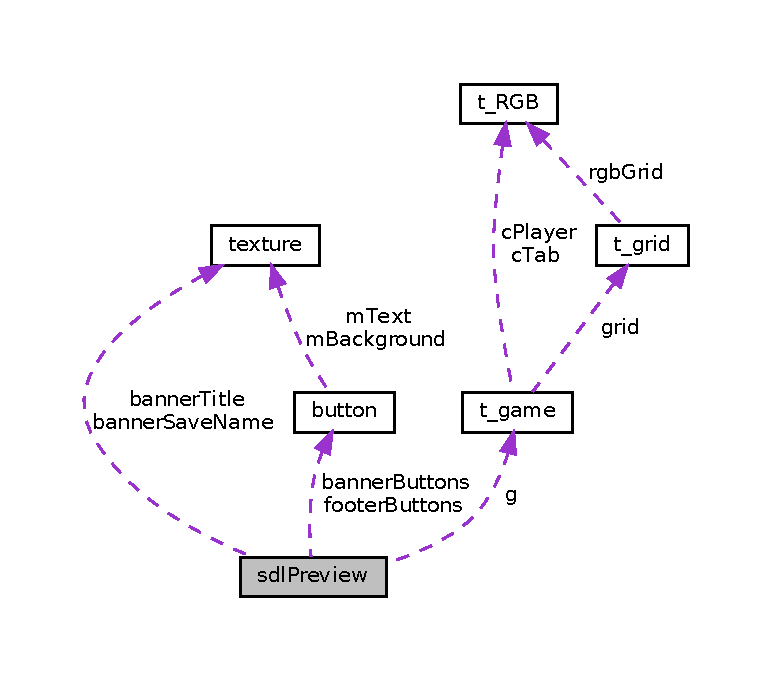
\includegraphics[width=350pt]{structsdl_preview__coll__graph}
\end{center}
\end{figure}
\subsection*{Data Fields}
\begin{DoxyCompactItemize}
\item 
\mbox{\Hypertarget{structsdl_preview_a04da60f12d502931bdcc034cad86347f}\label{structsdl_preview_a04da60f12d502931bdcc034cad86347f}} 
S\+D\+L\+\_\+\+Window $\ast$$\ast$ {\bfseries g\+Window}
\item 
\mbox{\Hypertarget{structsdl_preview_ad916adf6a3c707eda83ceefbdee69a26}\label{structsdl_preview_ad916adf6a3c707eda83ceefbdee69a26}} 
S\+D\+L\+\_\+\+Renderer $\ast$$\ast$ {\bfseries g\+Renderer}
\item 
\mbox{\Hypertarget{structsdl_preview_abf5bfa705e66ffc1ddaa6ce46c960873}\label{structsdl_preview_abf5bfa705e66ffc1ddaa6ce46c960873}} 
T\+T\+F\+\_\+\+Font $\ast$ {\bfseries font}
\item 
\mbox{\Hypertarget{structsdl_preview_a3f3b791c64b074b7d315a41416fd452d}\label{structsdl_preview_a3f3b791c64b074b7d315a41416fd452d}} 
\hyperlink{structt__game}{game} $\ast$ {\bfseries g}
\item 
\mbox{\Hypertarget{structsdl_preview_a326ac0832310ae96cbae0f489eedac92}\label{structsdl_preview_a326ac0832310ae96cbae0f489eedac92}} 
Game\+State {\bfseries gs}
\item 
\mbox{\Hypertarget{structsdl_preview_a0e572169338230e30d01a3b1af9324a1}\label{structsdl_preview_a0e572169338230e30d01a3b1af9324a1}} 
\hyperlink{structtexture}{L\+Texture} $\ast$ {\bfseries banner\+Title}
\item 
\mbox{\Hypertarget{structsdl_preview_afc05f8d61660f4e5a5cdd42ad5b365a6}\label{structsdl_preview_afc05f8d61660f4e5a5cdd42ad5b365a6}} 
\hyperlink{structtexture}{L\+Texture} $\ast$ {\bfseries banner\+Save\+Name}
\item 
\mbox{\Hypertarget{structsdl_preview_a898a14b8dbc4ff8f956752cbd5df0aab}\label{structsdl_preview_a898a14b8dbc4ff8f956752cbd5df0aab}} 
\hyperlink{structbutton}{L\+Button} $\ast$ {\bfseries banner\+Buttons} \mbox{[}2\mbox{]}
\item 
\mbox{\Hypertarget{structsdl_preview_aead1c01f276e85f212e16ce43e14fb14}\label{structsdl_preview_aead1c01f276e85f212e16ce43e14fb14}} 
\hyperlink{structbutton}{L\+Button} $\ast$ {\bfseries footer\+Buttons} \mbox{[}3\mbox{]}
\item 
\mbox{\Hypertarget{structsdl_preview_a8f92c2e25faedfc1bd2f8bbcc9800367}\label{structsdl_preview_a8f92c2e25faedfc1bd2f8bbcc9800367}} 
int {\bfseries saves\+Count}
\item 
\mbox{\Hypertarget{structsdl_preview_a35a2f07034a53e5087d2d1edfdbdc9f5}\label{structsdl_preview_a35a2f07034a53e5087d2d1edfdbdc9f5}} 
char $\ast$$\ast$ {\bfseries saves\+Names}
\item 
\mbox{\Hypertarget{structsdl_preview_a528aac3c388ec9fffe77578e5b569341}\label{structsdl_preview_a528aac3c388ec9fffe77578e5b569341}} 
int {\bfseries current\+Save}
\end{DoxyCompactItemize}


The documentation for this struct was generated from the following file\+:\begin{DoxyCompactItemize}
\item 
src/sdl/game\+\_\+load\+\_\+rendering.\+h\end{DoxyCompactItemize}

\hypertarget{structsettings_screen}{}\section{settings\+Screen Struct Reference}
\label{structsettings_screen}\index{settings\+Screen@{settings\+Screen}}


Collaboration diagram for settings\+Screen\+:
\nopagebreak
\begin{figure}[H]
\begin{center}
\leavevmode
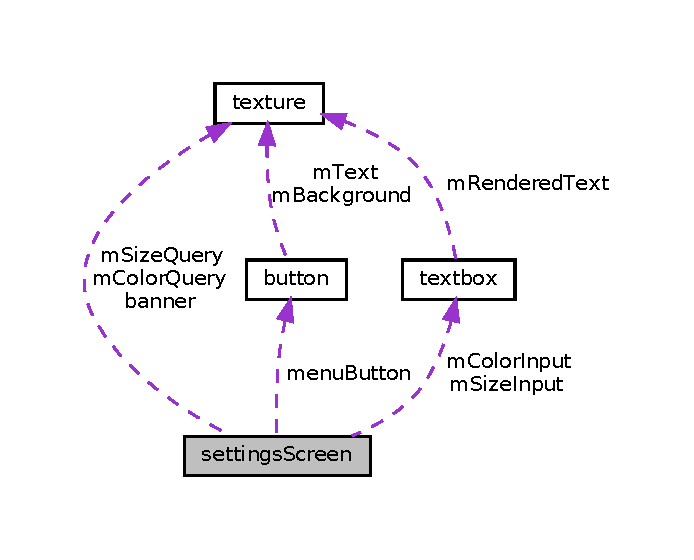
\includegraphics[width=333pt]{structsettings_screen__coll__graph}
\end{center}
\end{figure}
\subsection*{Data Fields}
\begin{DoxyCompactItemize}
\item 
\mbox{\Hypertarget{structsettings_screen_a068d01584474022d1049f78565d551f9}\label{structsettings_screen_a068d01584474022d1049f78565d551f9}} 
\hyperlink{structtexture}{L\+Texture} $\ast$ {\bfseries banner}
\item 
\mbox{\Hypertarget{structsettings_screen_a672a362d05743dccdde0fec4e95156f8}\label{structsettings_screen_a672a362d05743dccdde0fec4e95156f8}} 
int $\ast$ {\bfseries board\+Size}
\item 
\mbox{\Hypertarget{structsettings_screen_ac21e6b079e5191b7a42f90096b6d213e}\label{structsettings_screen_ac21e6b079e5191b7a42f90096b6d213e}} 
int $\ast$ {\bfseries color\+Amount}
\item 
\mbox{\Hypertarget{structsettings_screen_a166b9c7b6f9424d5d22a7c5306c24d01}\label{structsettings_screen_a166b9c7b6f9424d5d22a7c5306c24d01}} 
\hyperlink{structtexture}{L\+Texture} $\ast$ {\bfseries m\+Size\+Query}
\item 
\mbox{\Hypertarget{structsettings_screen_a720b673a2957e44d181b85a28f04eba4}\label{structsettings_screen_a720b673a2957e44d181b85a28f04eba4}} 
\hyperlink{structtextbox}{L\+Textbox} $\ast$ {\bfseries m\+Size\+Input}
\item 
\mbox{\Hypertarget{structsettings_screen_ab4a50251d5ca99b28a59dd5e0fb43e83}\label{structsettings_screen_ab4a50251d5ca99b28a59dd5e0fb43e83}} 
\hyperlink{structtexture}{L\+Texture} $\ast$ {\bfseries m\+Color\+Query}
\item 
\mbox{\Hypertarget{structsettings_screen_ac950a41138dc6610dfa1e0dcc6ca46a9}\label{structsettings_screen_ac950a41138dc6610dfa1e0dcc6ca46a9}} 
\hyperlink{structtextbox}{L\+Textbox} $\ast$ {\bfseries m\+Color\+Input}
\item 
\mbox{\Hypertarget{structsettings_screen_abd981fb6e197d0155c00e3bc92703198}\label{structsettings_screen_abd981fb6e197d0155c00e3bc92703198}} 
\hyperlink{structbutton}{L\+Button} $\ast$ {\bfseries menu\+Button}
\item 
\mbox{\Hypertarget{structsettings_screen_a326ac0832310ae96cbae0f489eedac92}\label{structsettings_screen_a326ac0832310ae96cbae0f489eedac92}} 
Game\+State {\bfseries gs}
\end{DoxyCompactItemize}


The documentation for this struct was generated from the following file\+:\begin{DoxyCompactItemize}
\item 
src/sdl/game\+\_\+settings\+\_\+rendering.\+h\end{DoxyCompactItemize}

\hypertarget{structt__game}{}\section{t\+\_\+game Struct Reference}
\label{structt__game}\index{t\+\_\+game@{t\+\_\+game}}


Structure de la partie.  




{\ttfamily \#include $<$game.\+h$>$}



Collaboration diagram for t\+\_\+game\+:
\nopagebreak
\begin{figure}[H]
\begin{center}
\leavevmode
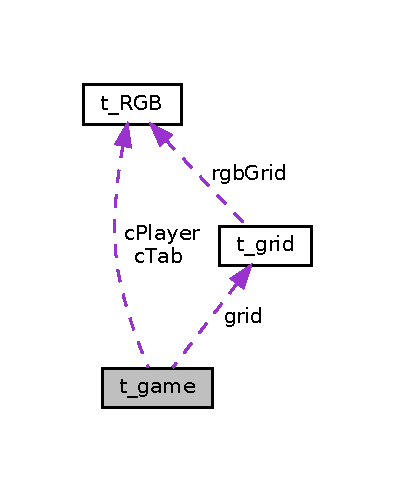
\includegraphics[width=190pt]{structt__game__coll__graph}
\end{center}
\end{figure}
\subsection*{Data Fields}
\begin{DoxyCompactItemize}
\item 
\mbox{\Hypertarget{structt__game_a780e12a56f86fb3822d28afec44c2685}\label{structt__game_a780e12a56f86fb3822d28afec44c2685}} 
\hyperlink{structt__grid}{grid} $\ast$ {\bfseries grid}
\item 
\mbox{\Hypertarget{structt__game_a439227feff9d7f55384e8780cfc2eb82}\label{structt__game_a439227feff9d7f55384e8780cfc2eb82}} 
int {\bfseries size}
\item 
\mbox{\Hypertarget{structt__game_a6a9496106a62415d229b9d57c6152a9b}\label{structt__game_a6a9496106a62415d229b9d57c6152a9b}} 
int {\bfseries c\+Nb}
\item 
\mbox{\Hypertarget{structt__game_ab71773449e39dc6d45e68234a5ff47f2}\label{structt__game_ab71773449e39dc6d45e68234a5ff47f2}} 
int {\bfseries turn\+Count}
\item 
\mbox{\Hypertarget{structt__game_af5e477e41902666eec462e69916b547d}\label{structt__game_af5e477e41902666eec462e69916b547d}} 
\hyperlink{structt___r_g_b}{R\+GB} $\ast$ {\bfseries c\+Tab}
\item 
\mbox{\Hypertarget{structt__game_a46ffdfb273ea74bbb8a3df3ae0f00897}\label{structt__game_a46ffdfb273ea74bbb8a3df3ae0f00897}} 
\hyperlink{structt___r_g_b}{R\+GB} {\bfseries c\+Player}
\end{DoxyCompactItemize}


\subsection{Detailed Description}
Structure de la partie. 

The documentation for this struct was generated from the following file\+:\begin{DoxyCompactItemize}
\item 
src/game/game.\+h\end{DoxyCompactItemize}

\hypertarget{structt__grid}{}\section{t\+\_\+grid Struct Reference}
\label{structt__grid}\index{t\+\_\+grid@{t\+\_\+grid}}


Structure d\textquotesingle{}une grille.  




{\ttfamily \#include $<$grid.\+h$>$}



Collaboration diagram for t\+\_\+grid\+:
\nopagebreak
\begin{figure}[H]
\begin{center}
\leavevmode
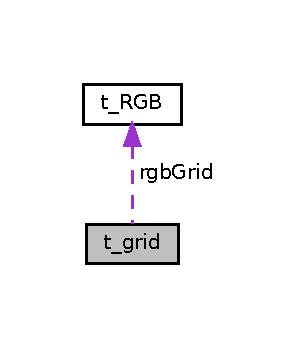
\includegraphics[width=144pt]{structt__grid__coll__graph}
\end{center}
\end{figure}
\subsection*{Data Fields}
\begin{DoxyCompactItemize}
\item 
\mbox{\Hypertarget{structt__grid_aa6f2a52326d2c1cbac9582f07c863527}\label{structt__grid_aa6f2a52326d2c1cbac9582f07c863527}} 
\hyperlink{structt___r_g_b}{R\+GB} $\ast$ {\bfseries rgb\+Grid}
\item 
\mbox{\Hypertarget{structt__grid_ae9a300bb716cd15c538cbf00aa6db8f9}\label{structt__grid_ae9a300bb716cd15c538cbf00aa6db8f9}} 
int $\ast$ {\bfseries cc\+Grid}
\item 
\mbox{\Hypertarget{structt__grid_a439227feff9d7f55384e8780cfc2eb82}\label{structt__grid_a439227feff9d7f55384e8780cfc2eb82}} 
int {\bfseries size}
\item 
\mbox{\Hypertarget{structt__grid_aed485617e262f55fd47a014bdcb6e2a0}\label{structt__grid_aed485617e262f55fd47a014bdcb6e2a0}} 
int {\bfseries max\+Label}
\end{DoxyCompactItemize}


\subsection{Detailed Description}
Structure d\textquotesingle{}une grille. 

The documentation for this struct was generated from the following file\+:\begin{DoxyCompactItemize}
\item 
src/game/grid.\+h\end{DoxyCompactItemize}

\hypertarget{structt___r_g_b}{}\section{t\+\_\+\+R\+GB Struct Reference}
\label{structt___r_g_b}\index{t\+\_\+\+R\+GB@{t\+\_\+\+R\+GB}}


Structure d\textquotesingle{}une couleur en utilisant le code rgb.  




{\ttfamily \#include $<$rgb.\+h$>$}

\subsection*{Data Fields}
\begin{DoxyCompactItemize}
\item 
\mbox{\Hypertarget{structt___r_g_b_a99b994edd82192c4fe92f1699f3c1085}\label{structt___r_g_b_a99b994edd82192c4fe92f1699f3c1085}} 
unsigned char {\bfseries R}
\item 
\mbox{\Hypertarget{structt___r_g_b_a9ceb27cca5e312d4e16505213eb76661}\label{structt___r_g_b_a9ceb27cca5e312d4e16505213eb76661}} 
unsigned char {\bfseries G}
\item 
\mbox{\Hypertarget{structt___r_g_b_a8c81a457ae49e23c5e69f9d79bbd1131}\label{structt___r_g_b_a8c81a457ae49e23c5e69f9d79bbd1131}} 
unsigned char {\bfseries B}
\end{DoxyCompactItemize}


\subsection{Detailed Description}
Structure d\textquotesingle{}une couleur en utilisant le code rgb. 

The documentation for this struct was generated from the following file\+:\begin{DoxyCompactItemize}
\item 
src/game/rgb.\+h\end{DoxyCompactItemize}

\hypertarget{structtextbox}{}\section{textbox Struct Reference}
\label{structtextbox}\index{textbox@{textbox}}


Collaboration diagram for textbox\+:
\nopagebreak
\begin{figure}[H]
\begin{center}
\leavevmode
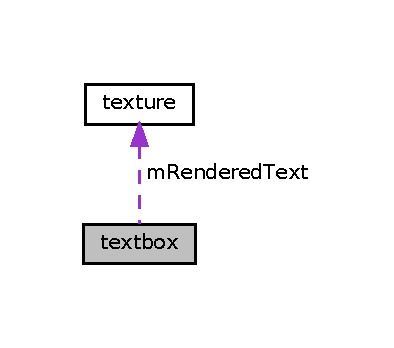
\includegraphics[width=189pt]{structtextbox__coll__graph}
\end{center}
\end{figure}
\subsection*{Data Fields}
\begin{DoxyCompactItemize}
\item 
\mbox{\Hypertarget{structtextbox_a7effa71f13f562fc3a9e174b4a3dd678}\label{structtextbox_a7effa71f13f562fc3a9e174b4a3dd678}} 
char $\ast$ {\bfseries m\+Text}
\item 
\mbox{\Hypertarget{structtextbox_afaf5ffcd96533dfa98e030421fcb78cc}\label{structtextbox_afaf5ffcd96533dfa98e030421fcb78cc}} 
int {\bfseries m\+Text\+Length}
\item 
\mbox{\Hypertarget{structtextbox_a55d71a9c7b9d9b59fd061fd732e5b673}\label{structtextbox_a55d71a9c7b9d9b59fd061fd732e5b673}} 
\hyperlink{structtexture}{L\+Texture} $\ast$ {\bfseries m\+Rendered\+Text}
\item 
\mbox{\Hypertarget{structtextbox_a565fe26ba3de4ef01d9d6a4b6b6725d2}\label{structtextbox_a565fe26ba3de4ef01d9d6a4b6b6725d2}} 
S\+D\+L\+\_\+\+Point {\bfseries m\+Position}
\item 
\mbox{\Hypertarget{structtextbox_aa7b1c5aa09d5a6d8db57bf1481aa83e0}\label{structtextbox_aa7b1c5aa09d5a6d8db57bf1481aa83e0}} 
textbox\+State {\bfseries ts}
\end{DoxyCompactItemize}


The documentation for this struct was generated from the following file\+:\begin{DoxyCompactItemize}
\item 
src/sdl/textbox\+\_\+wrapper.\+h\end{DoxyCompactItemize}

\hypertarget{structtexture}{}\section{texture Struct Reference}
\label{structtexture}\index{texture@{texture}}
\subsection*{Data Fields}
\begin{DoxyCompactItemize}
\item 
\mbox{\Hypertarget{structtexture_a13441ecc6f09930e330ecc4b48189778}\label{structtexture_a13441ecc6f09930e330ecc4b48189778}} 
S\+D\+L\+\_\+\+Texture $\ast$ {\bfseries m\+Texture}
\item 
\mbox{\Hypertarget{structtexture_aa39f004a83a206ca8644d441c792e45b}\label{structtexture_aa39f004a83a206ca8644d441c792e45b}} 
int {\bfseries m\+Width}
\item 
\mbox{\Hypertarget{structtexture_a3d6a057795437ab1becbd09b09ea7a90}\label{structtexture_a3d6a057795437ab1becbd09b09ea7a90}} 
int {\bfseries m\+Height}
\item 
\mbox{\Hypertarget{structtexture_abf5bfa705e66ffc1ddaa6ce46c960873}\label{structtexture_abf5bfa705e66ffc1ddaa6ce46c960873}} 
T\+T\+F\+\_\+\+Font $\ast$ {\bfseries font}
\item 
\mbox{\Hypertarget{structtexture_a04da60f12d502931bdcc034cad86347f}\label{structtexture_a04da60f12d502931bdcc034cad86347f}} 
S\+D\+L\+\_\+\+Window $\ast$$\ast$ {\bfseries g\+Window}
\item 
\mbox{\Hypertarget{structtexture_ad916adf6a3c707eda83ceefbdee69a26}\label{structtexture_ad916adf6a3c707eda83ceefbdee69a26}} 
S\+D\+L\+\_\+\+Renderer $\ast$$\ast$ {\bfseries g\+Renderer}
\end{DoxyCompactItemize}


The documentation for this struct was generated from the following file\+:\begin{DoxyCompactItemize}
\item 
src/sdl/texture\+\_\+wrapper.\+h\end{DoxyCompactItemize}

\chapter{File Documentation}
\hypertarget{game_8c}{}\section{src/game/game.c File Reference}
\label{game_8c}\index{src/game/game.\+c@{src/game/game.\+c}}


Gestion du jeu pendant une partie.  


{\ttfamily \#include \char`\"{}game.\+h\char`\"{}}\newline
Include dependency graph for game.\+c\+:
\nopagebreak
\begin{figure}[H]
\begin{center}
\leavevmode
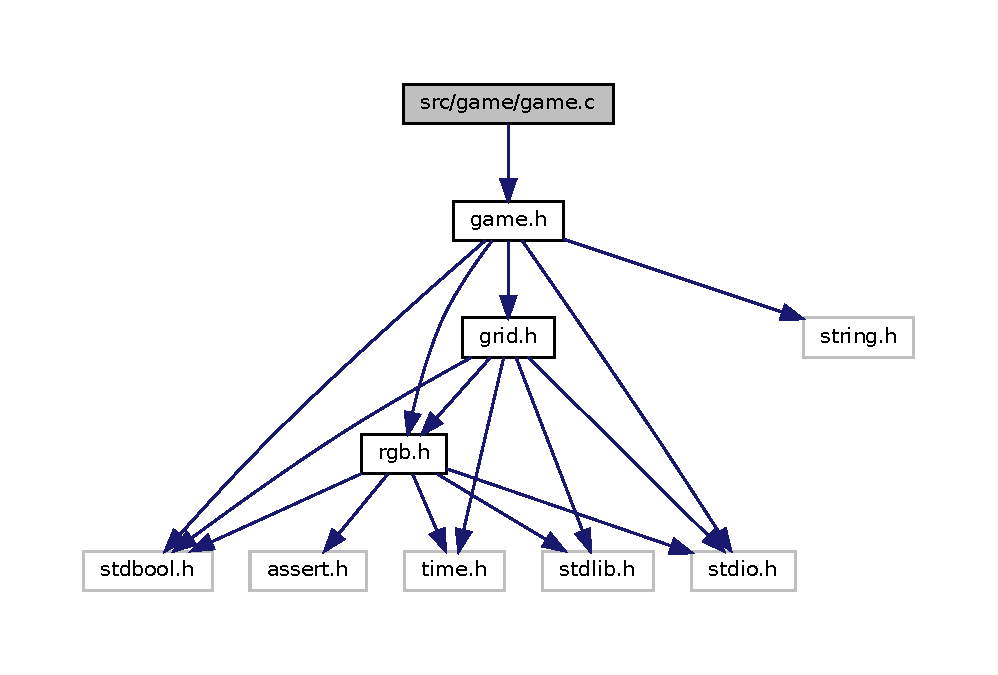
\includegraphics[width=350pt]{game_8c__incl}
\end{center}
\end{figure}
\subsection*{Functions}
\begin{DoxyCompactItemize}
\item 
\hyperlink{structt__game}{game} $\ast$ \hyperlink{game_8c_a887f37f53d21c0daee1b6ef659232c41}{game\+Init} (int size, int c\+Nb)
\begin{DoxyCompactList}\small\item\em Initialise une partie avec une grille qui contient un nombre donné de couleurs, générées au hasard. \end{DoxyCompactList}\item 
void \hyperlink{game_8c_a11118d44e944dbbfd45153619a3d9842}{game\+Print} (\hyperlink{structt__game}{game} $\ast$g)
\begin{DoxyCompactList}\small\item\em Affiche la grille de jeu et d\textquotesingle{}autres informations. \end{DoxyCompactList}\item 
void \hyperlink{game_8c_a189935d1d9e3b825791ddf76483de4a9}{game\+Free} (\hyperlink{structt__game}{game} $\ast$g)
\begin{DoxyCompactList}\small\item\em Supprime la partie. \end{DoxyCompactList}\item 
void \hyperlink{game_8c_a7636217618dfe710f503a86c8ccae3a7}{game\+Play\+Turn} (\hyperlink{structt__game}{game} $\ast$g)
\begin{DoxyCompactList}\small\item\em Modifie la grille après que le joueur ait décidé d\textquotesingle{}une couleur. \end{DoxyCompactList}\item 
void \hyperlink{game_8c_ac7cd8a7483961d1874ee746da58dd6dd}{game\+Play\+Turn\+S\+DL} (\hyperlink{structt__game}{game} $\ast$g, int new\+Color)
\begin{DoxyCompactList}\small\item\em Modifie la grille en jouant la couleur new\+Color (utilisé par l\textquotesingle{}interface game\+\_\+board\+\_\+rendering. \end{DoxyCompactList}\item 
bool \hyperlink{game_8c_a380255be34c051d613fd38a09935e0f0}{game\+Over} (\hyperlink{structt__game}{game} $\ast$g)
\begin{DoxyCompactList}\small\item\em Teste si la partie est terminée (victoire du joueur) ou si elle continue. \end{DoxyCompactList}\item 
\mbox{\Hypertarget{game_8c_aab77338d2fac882fd2aae7a5095d03d9}\label{game_8c_aab77338d2fac882fd2aae7a5095d03d9}} 
\hyperlink{structt__game}{game} $\ast$ {\bfseries game\+Import} (char $\ast$save)
\item 
\mbox{\Hypertarget{game_8c_a966bf18caafe6c97ccdd7bf5c30467fa}\label{game_8c_a966bf18caafe6c97ccdd7bf5c30467fa}} 
void {\bfseries game\+Export} (\hyperlink{structt__game}{game} $\ast$g)
\end{DoxyCompactItemize}


\subsection{Detailed Description}
Gestion du jeu pendant une partie. 

\begin{DoxyAuthor}{Author}
Last\+But\+Not\+Least 
\end{DoxyAuthor}
\begin{DoxyDate}{Date}
Mars 2017 
\end{DoxyDate}


\subsection{Function Documentation}
\mbox{\Hypertarget{game_8c_a189935d1d9e3b825791ddf76483de4a9}\label{game_8c_a189935d1d9e3b825791ddf76483de4a9}} 
\index{game.\+c@{game.\+c}!game\+Free@{game\+Free}}
\index{game\+Free@{game\+Free}!game.\+c@{game.\+c}}
\subsubsection{\texorpdfstring{game\+Free()}{gameFree()}}
{\footnotesize\ttfamily game\+Free (\begin{DoxyParamCaption}\item[{\hyperlink{structt__game}{game} $\ast$}]{g }\end{DoxyParamCaption})}



Supprime la partie. 


\begin{DoxyParams}{Parameters}
{\em g} & \+: le jeu \\
\hline
\end{DoxyParams}
Here is the call graph for this function\+:
\nopagebreak
\begin{figure}[H]
\begin{center}
\leavevmode
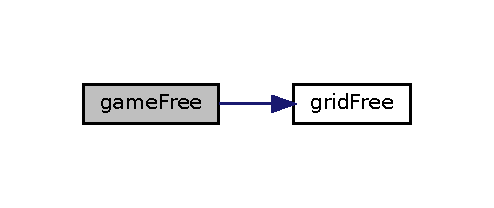
\includegraphics[width=237pt]{game_8c_a189935d1d9e3b825791ddf76483de4a9_cgraph}
\end{center}
\end{figure}
\mbox{\Hypertarget{game_8c_a887f37f53d21c0daee1b6ef659232c41}\label{game_8c_a887f37f53d21c0daee1b6ef659232c41}} 
\index{game.\+c@{game.\+c}!game\+Init@{game\+Init}}
\index{game\+Init@{game\+Init}!game.\+c@{game.\+c}}
\subsubsection{\texorpdfstring{game\+Init()}{gameInit()}}
{\footnotesize\ttfamily game\+Init (\begin{DoxyParamCaption}\item[{int}]{size,  }\item[{int}]{c\+Nb }\end{DoxyParamCaption})}



Initialise une partie avec une grille qui contient un nombre donné de couleurs, générées au hasard. 


\begin{DoxyParams}{Parameters}
{\em size} & \+: taille de la grille à générer ie nombre de cases d\textquotesingle{}un coté \\
\hline
{\em c\+Nb} & \+: Nombre de couleurs différentes \\
\hline
\end{DoxyParams}
\begin{DoxyReturn}{Returns}
Le jeu généré. 
\end{DoxyReturn}
Here is the call graph for this function\+:
\nopagebreak
\begin{figure}[H]
\begin{center}
\leavevmode
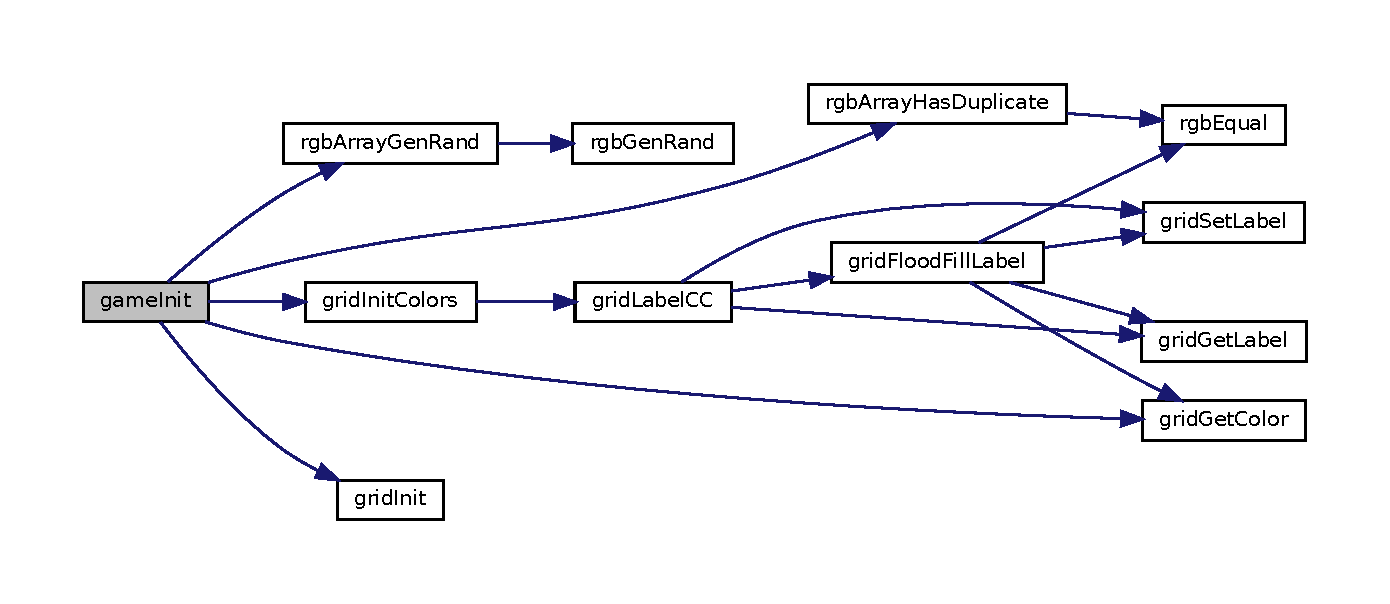
\includegraphics[width=350pt]{game_8c_a887f37f53d21c0daee1b6ef659232c41_cgraph}
\end{center}
\end{figure}
\mbox{\Hypertarget{game_8c_a380255be34c051d613fd38a09935e0f0}\label{game_8c_a380255be34c051d613fd38a09935e0f0}} 
\index{game.\+c@{game.\+c}!game\+Over@{game\+Over}}
\index{game\+Over@{game\+Over}!game.\+c@{game.\+c}}
\subsubsection{\texorpdfstring{game\+Over()}{gameOver()}}
{\footnotesize\ttfamily game\+Over (\begin{DoxyParamCaption}\item[{\hyperlink{structt__game}{game} $\ast$}]{g }\end{DoxyParamCaption})}



Teste si la partie est terminée (victoire du joueur) ou si elle continue. 


\begin{DoxyParams}{Parameters}
{\em g} & \+: le jeu \\
\hline
\end{DoxyParams}
\begin{DoxyReturn}{Returns}
true si le jeu est terminé, false sinon 
\end{DoxyReturn}
Here is the call graph for this function\+:
\nopagebreak
\begin{figure}[H]
\begin{center}
\leavevmode
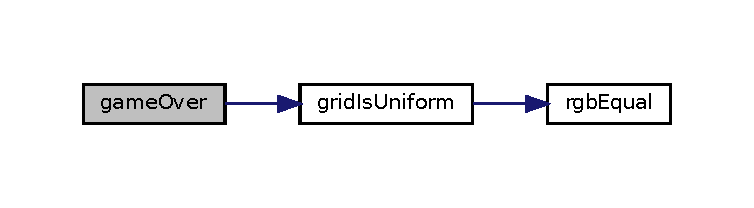
\includegraphics[width=350pt]{game_8c_a380255be34c051d613fd38a09935e0f0_cgraph}
\end{center}
\end{figure}
\mbox{\Hypertarget{game_8c_a7636217618dfe710f503a86c8ccae3a7}\label{game_8c_a7636217618dfe710f503a86c8ccae3a7}} 
\index{game.\+c@{game.\+c}!game\+Play\+Turn@{game\+Play\+Turn}}
\index{game\+Play\+Turn@{game\+Play\+Turn}!game.\+c@{game.\+c}}
\subsubsection{\texorpdfstring{game\+Play\+Turn()}{gamePlayTurn()}}
{\footnotesize\ttfamily game\+Play\+Turn (\begin{DoxyParamCaption}\item[{\hyperlink{structt__game}{game} $\ast$}]{g }\end{DoxyParamCaption})}



Modifie la grille après que le joueur ait décidé d\textquotesingle{}une couleur. 


\begin{DoxyParams}{Parameters}
{\em g} & \+: le jeu \\
\hline
\end{DoxyParams}
Here is the call graph for this function\+:
\nopagebreak
\begin{figure}[H]
\begin{center}
\leavevmode
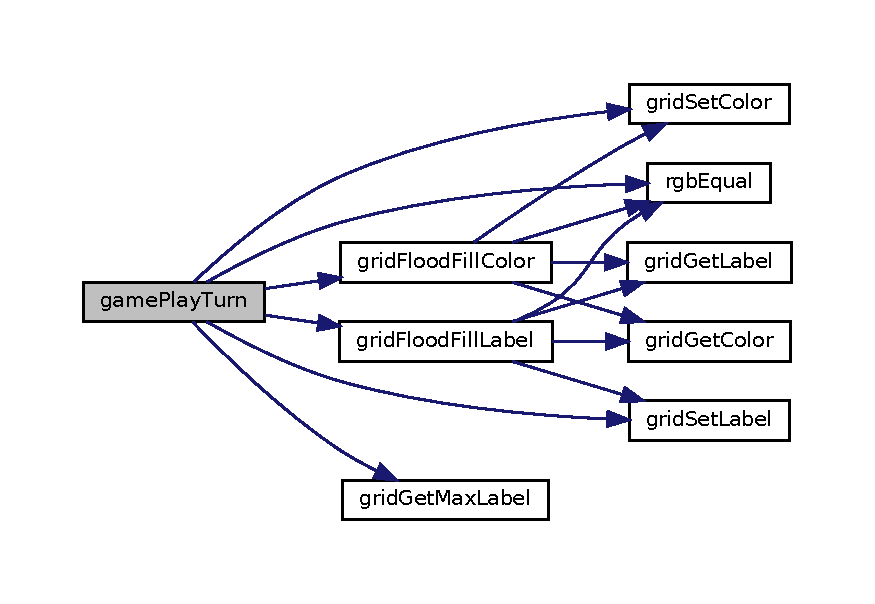
\includegraphics[width=350pt]{game_8c_a7636217618dfe710f503a86c8ccae3a7_cgraph}
\end{center}
\end{figure}
\mbox{\Hypertarget{game_8c_ac7cd8a7483961d1874ee746da58dd6dd}\label{game_8c_ac7cd8a7483961d1874ee746da58dd6dd}} 
\index{game.\+c@{game.\+c}!game\+Play\+Turn\+S\+DL@{game\+Play\+Turn\+S\+DL}}
\index{game\+Play\+Turn\+S\+DL@{game\+Play\+Turn\+S\+DL}!game.\+c@{game.\+c}}
\subsubsection{\texorpdfstring{game\+Play\+Turn\+S\+D\+L()}{gamePlayTurnSDL()}}
{\footnotesize\ttfamily game\+Play\+Turn\+S\+DL (\begin{DoxyParamCaption}\item[{\hyperlink{structt__game}{game} $\ast$}]{g,  }\item[{int}]{new\+Color }\end{DoxyParamCaption})}



Modifie la grille en jouant la couleur new\+Color (utilisé par l\textquotesingle{}interface game\+\_\+board\+\_\+rendering. 


\begin{DoxyParams}{Parameters}
{\em g} & \+: le jeu \\
\hline
{\em new\+Color} & \+: indice de la couleur a jouer \\
\hline
\end{DoxyParams}
Here is the call graph for this function\+:
\nopagebreak
\begin{figure}[H]
\begin{center}
\leavevmode
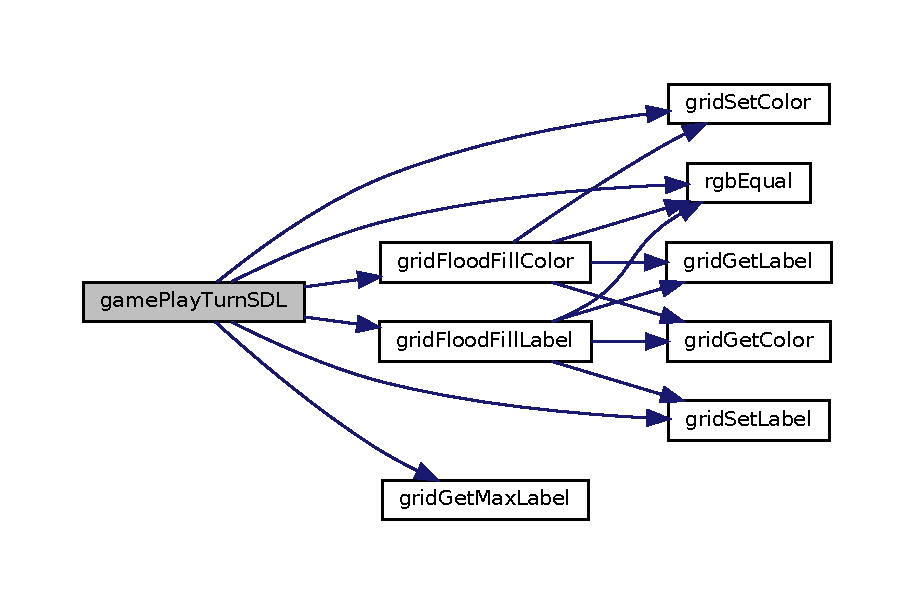
\includegraphics[width=350pt]{game_8c_ac7cd8a7483961d1874ee746da58dd6dd_cgraph}
\end{center}
\end{figure}
\mbox{\Hypertarget{game_8c_a11118d44e944dbbfd45153619a3d9842}\label{game_8c_a11118d44e944dbbfd45153619a3d9842}} 
\index{game.\+c@{game.\+c}!game\+Print@{game\+Print}}
\index{game\+Print@{game\+Print}!game.\+c@{game.\+c}}
\subsubsection{\texorpdfstring{game\+Print()}{gamePrint()}}
{\footnotesize\ttfamily game\+Print (\begin{DoxyParamCaption}\item[{\hyperlink{structt__game}{game} $\ast$}]{g }\end{DoxyParamCaption})}



Affiche la grille de jeu et d\textquotesingle{}autres informations. 


\begin{DoxyParams}{Parameters}
{\em g} & \+: le jeu \\
\hline
\end{DoxyParams}
Here is the call graph for this function\+:
\nopagebreak
\begin{figure}[H]
\begin{center}
\leavevmode
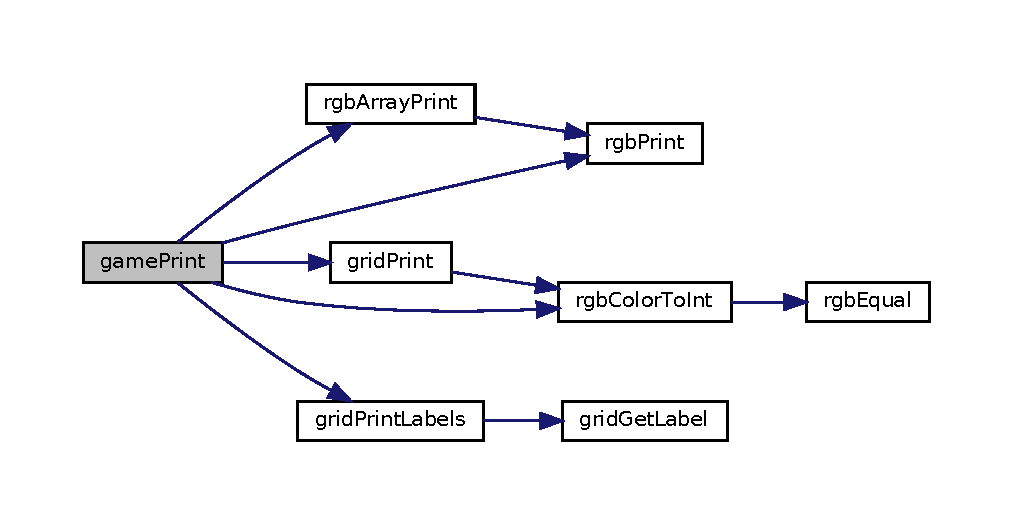
\includegraphics[width=350pt]{game_8c_a11118d44e944dbbfd45153619a3d9842_cgraph}
\end{center}
\end{figure}

\hypertarget{grid_8c}{}\section{src/game/grid.c File Reference}
\label{grid_8c}\index{src/game/grid.\+c@{src/game/grid.\+c}}


Gestion de la grille de jeu.  


{\ttfamily \#include \char`\"{}grid.\+h\char`\"{}}\newline
Include dependency graph for grid.\+c\+:
\nopagebreak
\begin{figure}[H]
\begin{center}
\leavevmode
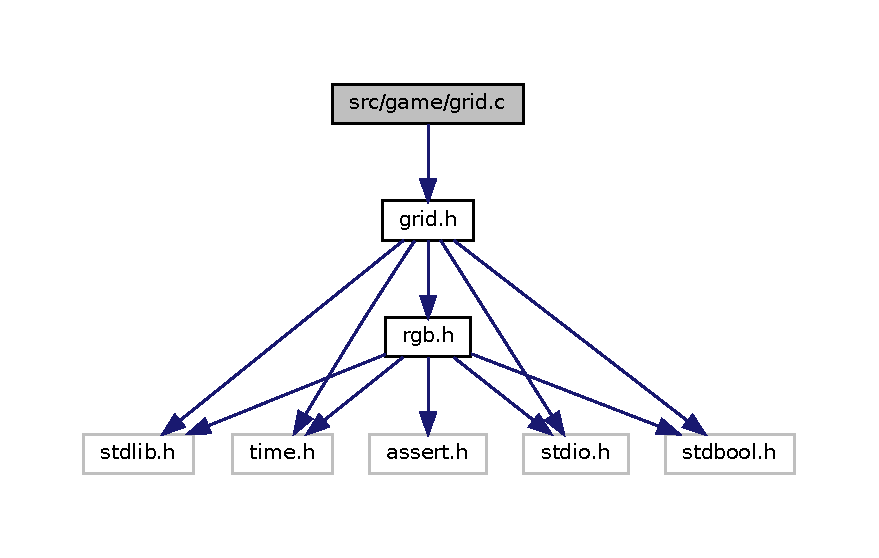
\includegraphics[width=350pt]{grid_8c__incl}
\end{center}
\end{figure}
\subsection*{Macros}
\begin{DoxyCompactItemize}
\item 
\mbox{\Hypertarget{grid_8c_aacc3ee1a7f283f8ef65cea31f4436a95}\label{grid_8c_aacc3ee1a7f283f8ef65cea31f4436a95}} 
\#define {\bfseries M\+AX}(x,  y)~(((x) $>$ (y)) ? (x) \+: (y))
\item 
\mbox{\Hypertarget{grid_8c_a74e75242132eaabbc1c512488a135926}\label{grid_8c_a74e75242132eaabbc1c512488a135926}} 
\#define {\bfseries M\+IN}(x,  y)~(((x) $<$ (y)) ? (x) \+: (y))
\end{DoxyCompactItemize}
\subsection*{Functions}
\begin{DoxyCompactItemize}
\item 
\hyperlink{structt__grid}{grid} $\ast$ \hyperlink{grid_8c_a8d8365e2dba2e31cc82d495f8542a393}{grid\+Init} (int size)
\begin{DoxyCompactList}\small\item\em Initialise une grille d\textquotesingle{}une taille donnée. \end{DoxyCompactList}\item 
void \hyperlink{grid_8c_a7b1a7fd47bc096b6430e02a4c2451e3f}{grid\+Init\+Colors} (\hyperlink{structt__grid}{grid} $\ast$g, \hyperlink{structt___r_g_b}{R\+GB} $\ast$c\+Tab, int c\+Nb)
\begin{DoxyCompactList}\small\item\em Génère des couleurs au hasard dans une grille, associe à chaque case son label et obtient le label maximal. \end{DoxyCompactList}\item 
\hyperlink{structt__grid}{grid} $\ast$ \hyperlink{grid_8c_a6e7e8c5d6e22b39ed1bde24783f13733}{grid\+Import} (F\+I\+LE $\ast$fp, int board\+\_\+size, \hyperlink{structt___r_g_b}{R\+GB} $\ast$c\+Tab, int c\+Nb)
\begin{DoxyCompactList}\small\item\em Importe une grille à partir d\textquotesingle{}un fichier existant. \end{DoxyCompactList}\item 
void \hyperlink{grid_8c_a2050f3ba54b5a9efa6d7fea841d98bae}{grid\+Export} (F\+I\+LE $\ast$fp, \hyperlink{structt__grid}{grid} $\ast$g, \hyperlink{structt___r_g_b}{R\+GB} $\ast$c\+Tab, int c\+Nb)
\begin{DoxyCompactList}\small\item\em Exporte une grille dans un fichier. \end{DoxyCompactList}\item 
\hyperlink{structt___r_g_b}{R\+GB} \hyperlink{grid_8c_a4d6f2609a0e5c49bd539a3f39f3208e5}{grid\+Get\+Color} (\hyperlink{structt__grid}{grid} $\ast$g, int x, int y)
\begin{DoxyCompactList}\small\item\em Donne la couleur d\textquotesingle{}une case d\textquotesingle{}une grille. \end{DoxyCompactList}\item 
void \hyperlink{grid_8c_a81c316eaecce336147a01cc72ae90801}{grid\+Set\+Color} (\hyperlink{structt__grid}{grid} $\ast$g, \hyperlink{structt___r_g_b}{R\+GB} new\+Color, int x, int y)
\begin{DoxyCompactList}\small\item\em Affecte une couleur à une case d\textquotesingle{}une grille. \end{DoxyCompactList}\item 
int \hyperlink{grid_8c_a42d5cd3f41ffe6bff0152df208a9d6b3}{grid\+Get\+Label} (\hyperlink{structt__grid}{grid} $\ast$g, int x, int y)
\begin{DoxyCompactList}\small\item\em Obtient le label d\textquotesingle{}une case de la grille. \end{DoxyCompactList}\item 
void \hyperlink{grid_8c_a9915684f28fcfbfab54b8cb8cc019057}{grid\+Set\+Label} (\hyperlink{structt__grid}{grid} $\ast$g, int new\+Label, int x, int y)
\begin{DoxyCompactList}\small\item\em Associe un label à une case de la grille. \end{DoxyCompactList}\item 
int \hyperlink{grid_8c_a75aecdb01dc9eb7a2a796e0548ff41f8}{grid\+Get\+Max\+Label} (\hyperlink{structt__grid}{grid} $\ast$g)
\begin{DoxyCompactList}\small\item\em Obtient le plus grand label dans la grille. \end{DoxyCompactList}\item 
bool \hyperlink{grid_8c_a3377767dd9dd32fdb2568ddc5377742c}{grid\+Is\+Uniform} (\hyperlink{structt__grid}{grid} $\ast$g)
\begin{DoxyCompactList}\small\item\em Cherche si la grille est composée d\textquotesingle{}une seule couleur. \end{DoxyCompactList}\item 
void \hyperlink{grid_8c_abb571f3c21105ce908b464844e342c17}{grid\+Flood\+Fill\+Label} (\hyperlink{structt__grid}{grid} $\ast$g, int x, int y)
\begin{DoxyCompactList}\small\item\em Modifie le label de toutes les cases appartenant à la même composante connexe qu\textquotesingle{}une case visée, pour y associer le label de la case en question. \end{DoxyCompactList}\item 
void \hyperlink{grid_8c_a064f6dee42ce72a7118778eb127691a9}{grid\+Flood\+Fill\+Color} (\hyperlink{structt__grid}{grid} $\ast$g, int x, int y)
\begin{DoxyCompactList}\small\item\em Modifie la couleur de toutes les cases appartenant à la même composante connexe (ie même label) qu\textquotesingle{}une case visée, pour y associer la couleur de la case en question. \end{DoxyCompactList}\item 
int \hyperlink{grid_8c_ae8a514f42a0cf2a0c7b13d5194489a71}{grid\+Label\+CC} (\hyperlink{structt__grid}{grid} $\ast$g)
\begin{DoxyCompactList}\small\item\em Associe à chaque case un label (commun aux autres cases de la même composante connexe) et obtient le plus grand label. \end{DoxyCompactList}\item 
void \hyperlink{grid_8c_ad1e0b52bf8891e9090312f71e9cd5601}{grid\+Print} (\hyperlink{structt__grid}{grid} $\ast$g, \hyperlink{structt___r_g_b}{R\+GB} $\ast$c\+Tab, int c\+Nb)
\begin{DoxyCompactList}\small\item\em Affiche la grille \+: chaque case est représentée par le rang de sa couleur (comme élément du tableau de couleurs). \end{DoxyCompactList}\item 
void \hyperlink{grid_8c_ab3139f8df42186aa02e725f5bbf2431a}{grid\+Print\+Labels} (\hyperlink{structt__grid}{grid} $\ast$g)
\begin{DoxyCompactList}\small\item\em Affiche la grille \+: chaque case est représentée par son label. \end{DoxyCompactList}\item 
void \hyperlink{grid_8c_a2d4a237e32e2d86b6b14506de1385c99}{grid\+Free} (\hyperlink{structt__grid}{grid} $\ast$g)
\begin{DoxyCompactList}\small\item\em Supprime la grille. \end{DoxyCompactList}\end{DoxyCompactItemize}


\subsection{Detailed Description}
Gestion de la grille de jeu. 

\begin{DoxyAuthor}{Author}
Last\+But\+Not\+Least 
\end{DoxyAuthor}
\begin{DoxyDate}{Date}
Mars 2017 
\end{DoxyDate}


\subsection{Function Documentation}
\mbox{\Hypertarget{grid_8c_a2050f3ba54b5a9efa6d7fea841d98bae}\label{grid_8c_a2050f3ba54b5a9efa6d7fea841d98bae}} 
\index{grid.\+c@{grid.\+c}!grid\+Export@{grid\+Export}}
\index{grid\+Export@{grid\+Export}!grid.\+c@{grid.\+c}}
\subsubsection{\texorpdfstring{grid\+Export()}{gridExport()}}
{\footnotesize\ttfamily grid\+Export (\begin{DoxyParamCaption}\item[{F\+I\+LE $\ast$}]{fp,  }\item[{\hyperlink{structt__grid}{grid} $\ast$}]{g,  }\item[{\hyperlink{structt___r_g_b}{R\+GB} $\ast$}]{c\+Tab,  }\item[{int}]{c\+Nb }\end{DoxyParamCaption})}



Exporte une grille dans un fichier. 


\begin{DoxyParams}{Parameters}
{\em fp} & \+: le fichier \\
\hline
{\em g} & \+: la grille \\
\hline
{\em c\+Tab} & \+: tableau contenant les différentes couleurs \\
\hline
{\em c\+Nb} & \+: nombre de couleurs différentes \\
\hline
\end{DoxyParams}
Here is the call graph for this function\+:
\nopagebreak
\begin{figure}[H]
\begin{center}
\leavevmode
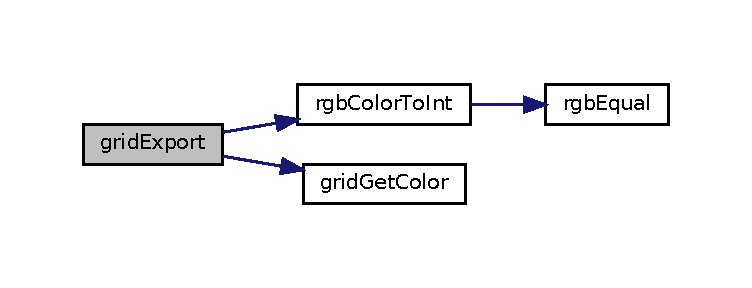
\includegraphics[width=350pt]{grid_8c_a2050f3ba54b5a9efa6d7fea841d98bae_cgraph}
\end{center}
\end{figure}
\mbox{\Hypertarget{grid_8c_a064f6dee42ce72a7118778eb127691a9}\label{grid_8c_a064f6dee42ce72a7118778eb127691a9}} 
\index{grid.\+c@{grid.\+c}!grid\+Flood\+Fill\+Color@{grid\+Flood\+Fill\+Color}}
\index{grid\+Flood\+Fill\+Color@{grid\+Flood\+Fill\+Color}!grid.\+c@{grid.\+c}}
\subsubsection{\texorpdfstring{grid\+Flood\+Fill\+Color()}{gridFloodFillColor()}}
{\footnotesize\ttfamily grid\+Flood\+Fill\+Color (\begin{DoxyParamCaption}\item[{\hyperlink{structt__grid}{grid} $\ast$}]{g,  }\item[{int}]{x,  }\item[{int}]{y }\end{DoxyParamCaption})}



Modifie la couleur de toutes les cases appartenant à la même composante connexe (ie même label) qu\textquotesingle{}une case visée, pour y associer la couleur de la case en question. 


\begin{DoxyParams}{Parameters}
{\em g} & \+: la grille \\
\hline
{\em x} & \+: numéro de la ligne qui contient la case visée \\
\hline
{\em y} & \+: numéro de la colonne qui contient la case visée \\
\hline
\end{DoxyParams}
Here is the call graph for this function\+:
\nopagebreak
\begin{figure}[H]
\begin{center}
\leavevmode
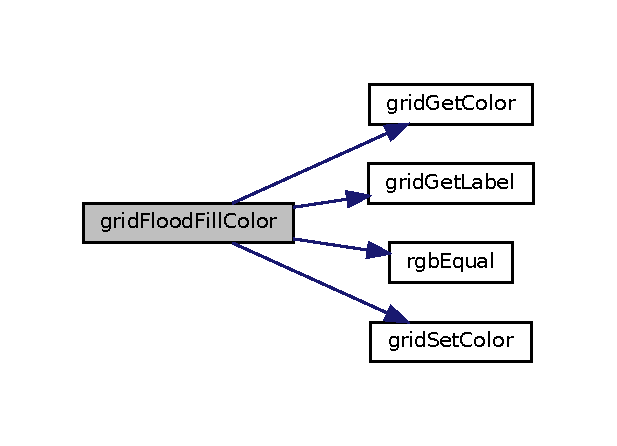
\includegraphics[width=296pt]{grid_8c_a064f6dee42ce72a7118778eb127691a9_cgraph}
\end{center}
\end{figure}
\mbox{\Hypertarget{grid_8c_abb571f3c21105ce908b464844e342c17}\label{grid_8c_abb571f3c21105ce908b464844e342c17}} 
\index{grid.\+c@{grid.\+c}!grid\+Flood\+Fill\+Label@{grid\+Flood\+Fill\+Label}}
\index{grid\+Flood\+Fill\+Label@{grid\+Flood\+Fill\+Label}!grid.\+c@{grid.\+c}}
\subsubsection{\texorpdfstring{grid\+Flood\+Fill\+Label()}{gridFloodFillLabel()}}
{\footnotesize\ttfamily grid\+Flood\+Fill\+Label (\begin{DoxyParamCaption}\item[{\hyperlink{structt__grid}{grid} $\ast$}]{g,  }\item[{int}]{x,  }\item[{int}]{y }\end{DoxyParamCaption})}



Modifie le label de toutes les cases appartenant à la même composante connexe qu\textquotesingle{}une case visée, pour y associer le label de la case en question. 


\begin{DoxyParams}{Parameters}
{\em g} & \+: la grille \\
\hline
{\em x} & \+: numéro de la ligne qui contient la case visée \\
\hline
{\em y} & \+: numéro de la colonne qui contient la case visée \\
\hline
\end{DoxyParams}
Here is the call graph for this function\+:
\nopagebreak
\begin{figure}[H]
\begin{center}
\leavevmode
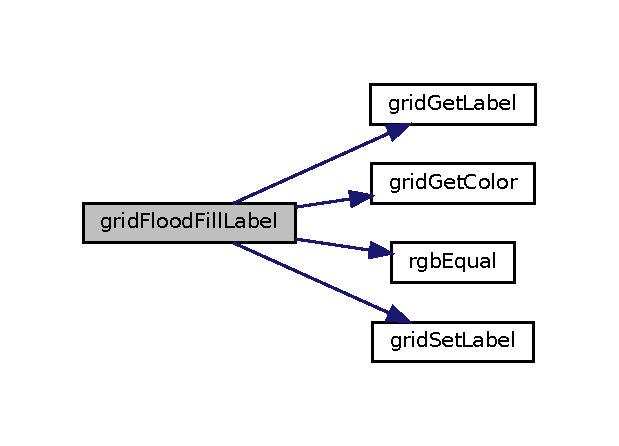
\includegraphics[width=297pt]{grid_8c_abb571f3c21105ce908b464844e342c17_cgraph}
\end{center}
\end{figure}
\mbox{\Hypertarget{grid_8c_a2d4a237e32e2d86b6b14506de1385c99}\label{grid_8c_a2d4a237e32e2d86b6b14506de1385c99}} 
\index{grid.\+c@{grid.\+c}!grid\+Free@{grid\+Free}}
\index{grid\+Free@{grid\+Free}!grid.\+c@{grid.\+c}}
\subsubsection{\texorpdfstring{grid\+Free()}{gridFree()}}
{\footnotesize\ttfamily grid\+Free (\begin{DoxyParamCaption}\item[{\hyperlink{structt__grid}{grid} $\ast$}]{g }\end{DoxyParamCaption})}



Supprime la grille. 


\begin{DoxyParams}{Parameters}
{\em g} & \+: la grille a supprimer \\
\hline
\end{DoxyParams}
\mbox{\Hypertarget{grid_8c_a4d6f2609a0e5c49bd539a3f39f3208e5}\label{grid_8c_a4d6f2609a0e5c49bd539a3f39f3208e5}} 
\index{grid.\+c@{grid.\+c}!grid\+Get\+Color@{grid\+Get\+Color}}
\index{grid\+Get\+Color@{grid\+Get\+Color}!grid.\+c@{grid.\+c}}
\subsubsection{\texorpdfstring{grid\+Get\+Color()}{gridGetColor()}}
{\footnotesize\ttfamily grid\+Get\+Color (\begin{DoxyParamCaption}\item[{\hyperlink{structt__grid}{grid} $\ast$}]{g,  }\item[{int}]{x,  }\item[{int}]{y }\end{DoxyParamCaption})}



Donne la couleur d\textquotesingle{}une case d\textquotesingle{}une grille. 


\begin{DoxyParams}{Parameters}
{\em g} & \+: la grille \\
\hline
{\em x} & \+: numéro de la colonne qui contient la case visée \\
\hline
{\em y} & \+: numéro de la ligne qui contient la case visée \\
\hline
\end{DoxyParams}
\begin{DoxyReturn}{Returns}
La couleur de la case en R\+GB 
\end{DoxyReturn}
\mbox{\Hypertarget{grid_8c_a42d5cd3f41ffe6bff0152df208a9d6b3}\label{grid_8c_a42d5cd3f41ffe6bff0152df208a9d6b3}} 
\index{grid.\+c@{grid.\+c}!grid\+Get\+Label@{grid\+Get\+Label}}
\index{grid\+Get\+Label@{grid\+Get\+Label}!grid.\+c@{grid.\+c}}
\subsubsection{\texorpdfstring{grid\+Get\+Label()}{gridGetLabel()}}
{\footnotesize\ttfamily grid\+Get\+Label (\begin{DoxyParamCaption}\item[{\hyperlink{structt__grid}{grid} $\ast$}]{g,  }\item[{int}]{x,  }\item[{int}]{y }\end{DoxyParamCaption})}



Obtient le label d\textquotesingle{}une case de la grille. 


\begin{DoxyParams}{Parameters}
{\em g} & \+: la grille \\
\hline
{\em x} & \+: numéro de la ligne qui contient la case visée \\
\hline
{\em y} & \+: numéro de la colonne qui contient la case visée \\
\hline
\end{DoxyParams}
\begin{DoxyReturn}{Returns}
Le numéro de la composante connexe de la case. 
\end{DoxyReturn}
\mbox{\Hypertarget{grid_8c_a75aecdb01dc9eb7a2a796e0548ff41f8}\label{grid_8c_a75aecdb01dc9eb7a2a796e0548ff41f8}} 
\index{grid.\+c@{grid.\+c}!grid\+Get\+Max\+Label@{grid\+Get\+Max\+Label}}
\index{grid\+Get\+Max\+Label@{grid\+Get\+Max\+Label}!grid.\+c@{grid.\+c}}
\subsubsection{\texorpdfstring{grid\+Get\+Max\+Label()}{gridGetMaxLabel()}}
{\footnotesize\ttfamily grid\+Get\+Max\+Label (\begin{DoxyParamCaption}\item[{\hyperlink{structt__grid}{grid} $\ast$}]{g }\end{DoxyParamCaption})}



Obtient le plus grand label dans la grille. 

Ce nombre n\textquotesingle{}est pas le nombre de labels dans la grille, et par conséquent pas le nombre de composantes connexes.


\begin{DoxyParams}{Parameters}
{\em g} & \+: la grille \\
\hline
\end{DoxyParams}
\begin{DoxyReturn}{Returns}
Le label maximal. 
\end{DoxyReturn}
\mbox{\Hypertarget{grid_8c_a6e7e8c5d6e22b39ed1bde24783f13733}\label{grid_8c_a6e7e8c5d6e22b39ed1bde24783f13733}} 
\index{grid.\+c@{grid.\+c}!grid\+Import@{grid\+Import}}
\index{grid\+Import@{grid\+Import}!grid.\+c@{grid.\+c}}
\subsubsection{\texorpdfstring{grid\+Import()}{gridImport()}}
{\footnotesize\ttfamily grid\+Import (\begin{DoxyParamCaption}\item[{F\+I\+LE $\ast$}]{fp,  }\item[{int}]{board\+\_\+size,  }\item[{\hyperlink{structt___r_g_b}{R\+GB} $\ast$}]{c\+Tab,  }\item[{int}]{c\+Nb }\end{DoxyParamCaption})}



Importe une grille à partir d\textquotesingle{}un fichier existant. 


\begin{DoxyParams}{Parameters}
{\em fp} & \+: le fichier \\
\hline
{\em board\+\_\+size} & \+: taille de la grille \\
\hline
{\em c\+Tab} & \+: tableau contenant les différentes couleurs \\
\hline
{\em c\+Nb} & \+: nombre de couleurs différentes \\
\hline
\end{DoxyParams}
\begin{DoxyReturn}{Returns}
la grille générée 
\end{DoxyReturn}
Here is the call graph for this function\+:
\nopagebreak
\begin{figure}[H]
\begin{center}
\leavevmode
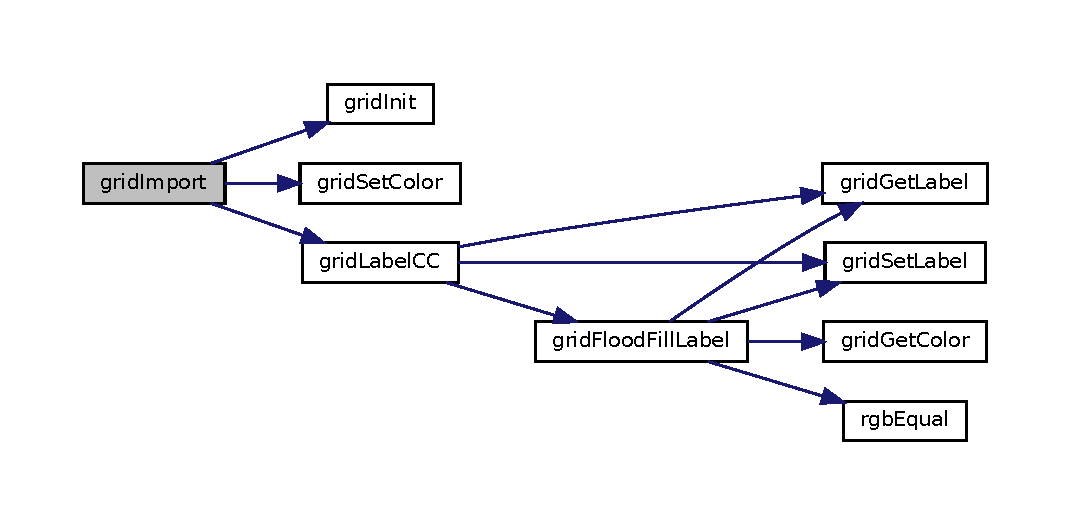
\includegraphics[width=350pt]{grid_8c_a6e7e8c5d6e22b39ed1bde24783f13733_cgraph}
\end{center}
\end{figure}
\mbox{\Hypertarget{grid_8c_a8d8365e2dba2e31cc82d495f8542a393}\label{grid_8c_a8d8365e2dba2e31cc82d495f8542a393}} 
\index{grid.\+c@{grid.\+c}!grid\+Init@{grid\+Init}}
\index{grid\+Init@{grid\+Init}!grid.\+c@{grid.\+c}}
\subsubsection{\texorpdfstring{grid\+Init()}{gridInit()}}
{\footnotesize\ttfamily grid\+Init (\begin{DoxyParamCaption}\item[{int}]{size }\end{DoxyParamCaption})}



Initialise une grille d\textquotesingle{}une taille donnée. 


\begin{DoxyParams}{Parameters}
{\em size} & \+: taille de la grille à générer ie nombre de cases d\textquotesingle{}un coté \\
\hline
\end{DoxyParams}
\begin{DoxyReturn}{Returns}
La grille générée. 
\end{DoxyReturn}
\mbox{\Hypertarget{grid_8c_a7b1a7fd47bc096b6430e02a4c2451e3f}\label{grid_8c_a7b1a7fd47bc096b6430e02a4c2451e3f}} 
\index{grid.\+c@{grid.\+c}!grid\+Init\+Colors@{grid\+Init\+Colors}}
\index{grid\+Init\+Colors@{grid\+Init\+Colors}!grid.\+c@{grid.\+c}}
\subsubsection{\texorpdfstring{grid\+Init\+Colors()}{gridInitColors()}}
{\footnotesize\ttfamily grid\+Init\+Colors (\begin{DoxyParamCaption}\item[{\hyperlink{structt__grid}{grid} $\ast$}]{g,  }\item[{\hyperlink{structt___r_g_b}{R\+GB} $\ast$}]{c\+Tab,  }\item[{int}]{c\+Nb }\end{DoxyParamCaption})}



Génère des couleurs au hasard dans une grille, associe à chaque case son label et obtient le label maximal. 


\begin{DoxyParams}{Parameters}
{\em g} & \+: la grille dans laquelle il faut mettre des couleurs \\
\hline
{\em c\+Tab} & \+: tableau contenant les couleurs en code R\+GB, dans lequel on va piocher \\
\hline
{\em c\+Nb} & \+: nombre de couleurs du tableau \\
\hline
\end{DoxyParams}
Here is the call graph for this function\+:
\nopagebreak
\begin{figure}[H]
\begin{center}
\leavevmode
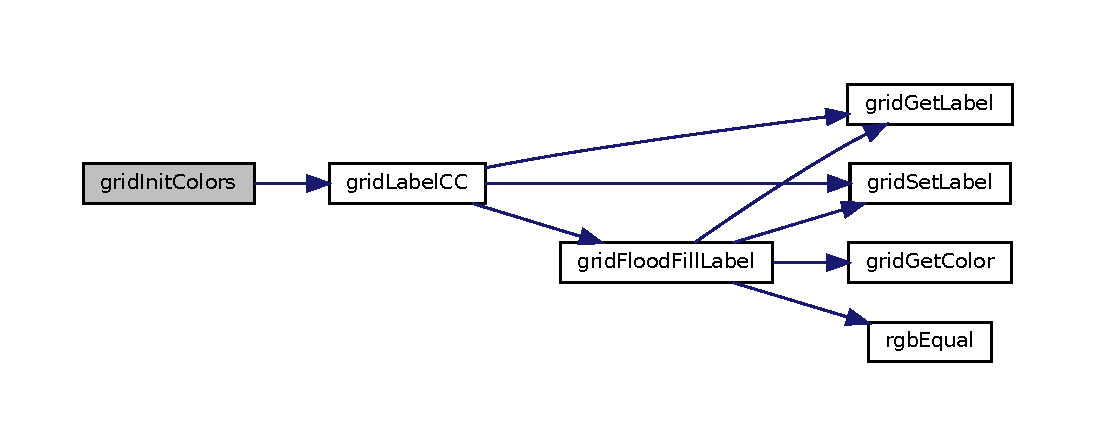
\includegraphics[width=350pt]{grid_8c_a7b1a7fd47bc096b6430e02a4c2451e3f_cgraph}
\end{center}
\end{figure}
\mbox{\Hypertarget{grid_8c_a3377767dd9dd32fdb2568ddc5377742c}\label{grid_8c_a3377767dd9dd32fdb2568ddc5377742c}} 
\index{grid.\+c@{grid.\+c}!grid\+Is\+Uniform@{grid\+Is\+Uniform}}
\index{grid\+Is\+Uniform@{grid\+Is\+Uniform}!grid.\+c@{grid.\+c}}
\subsubsection{\texorpdfstring{grid\+Is\+Uniform()}{gridIsUniform()}}
{\footnotesize\ttfamily grid\+Is\+Uniform (\begin{DoxyParamCaption}\item[{\hyperlink{structt__grid}{grid} $\ast$}]{g }\end{DoxyParamCaption})}



Cherche si la grille est composée d\textquotesingle{}une seule couleur. 


\begin{DoxyParams}{Parameters}
{\em g} & \+: la grille \\
\hline
\end{DoxyParams}
\begin{DoxyReturn}{Returns}
true si la grille est unicolore, false sinon. 
\end{DoxyReturn}
Here is the call graph for this function\+:
\nopagebreak
\begin{figure}[H]
\begin{center}
\leavevmode
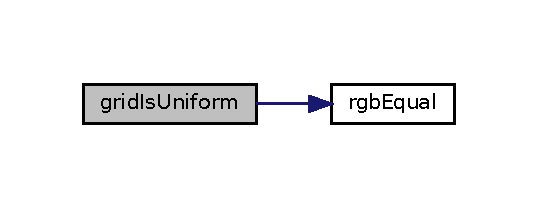
\includegraphics[width=258pt]{grid_8c_a3377767dd9dd32fdb2568ddc5377742c_cgraph}
\end{center}
\end{figure}
\mbox{\Hypertarget{grid_8c_ae8a514f42a0cf2a0c7b13d5194489a71}\label{grid_8c_ae8a514f42a0cf2a0c7b13d5194489a71}} 
\index{grid.\+c@{grid.\+c}!grid\+Label\+CC@{grid\+Label\+CC}}
\index{grid\+Label\+CC@{grid\+Label\+CC}!grid.\+c@{grid.\+c}}
\subsubsection{\texorpdfstring{grid\+Label\+C\+C()}{gridLabelCC()}}
{\footnotesize\ttfamily grid\+Label\+CC (\begin{DoxyParamCaption}\item[{\hyperlink{structt__grid}{grid} $\ast$}]{g }\end{DoxyParamCaption})}



Associe à chaque case un label (commun aux autres cases de la même composante connexe) et obtient le plus grand label. 

Le label maximal n\textquotesingle{}est pas le nombre de labels dans la grille, et par conséquent pas le nombre de composantes connexes


\begin{DoxyParams}{Parameters}
{\em g} & \+: la grille \\
\hline
\end{DoxyParams}
\begin{DoxyReturn}{Returns}
Le plus grand label 
\end{DoxyReturn}
Here is the call graph for this function\+:
\nopagebreak
\begin{figure}[H]
\begin{center}
\leavevmode
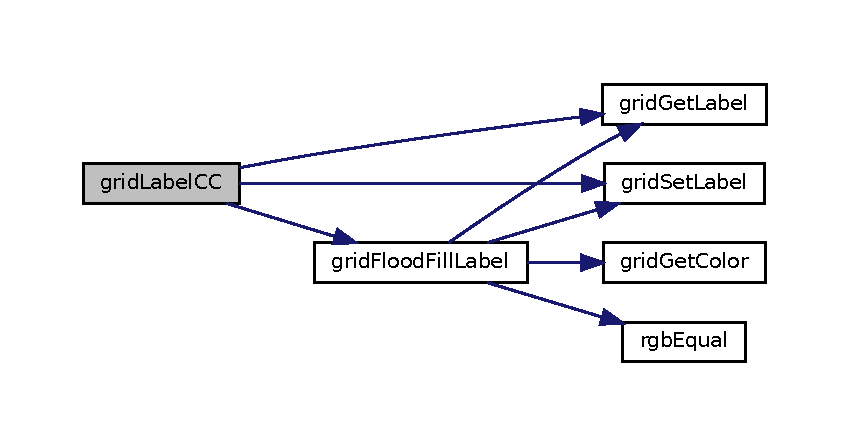
\includegraphics[width=350pt]{grid_8c_ae8a514f42a0cf2a0c7b13d5194489a71_cgraph}
\end{center}
\end{figure}
\mbox{\Hypertarget{grid_8c_ad1e0b52bf8891e9090312f71e9cd5601}\label{grid_8c_ad1e0b52bf8891e9090312f71e9cd5601}} 
\index{grid.\+c@{grid.\+c}!grid\+Print@{grid\+Print}}
\index{grid\+Print@{grid\+Print}!grid.\+c@{grid.\+c}}
\subsubsection{\texorpdfstring{grid\+Print()}{gridPrint()}}
{\footnotesize\ttfamily grid\+Print (\begin{DoxyParamCaption}\item[{\hyperlink{structt__grid}{grid} $\ast$}]{g,  }\item[{\hyperlink{structt___r_g_b}{R\+GB} $\ast$}]{c\+Tab,  }\item[{int}]{c\+Nb }\end{DoxyParamCaption})}



Affiche la grille \+: chaque case est représentée par le rang de sa couleur (comme élément du tableau de couleurs). 


\begin{DoxyParams}{Parameters}
{\em g} & \+: la grille \\
\hline
{\em c\+Tab} & \+: tableau contenant toutes les couleurs en code R\+GB \\
\hline
{\em c\+Nb} & \+: nombre de couleurs différentes contenues dans le tableau \\
\hline
\end{DoxyParams}
Here is the call graph for this function\+:
\nopagebreak
\begin{figure}[H]
\begin{center}
\leavevmode
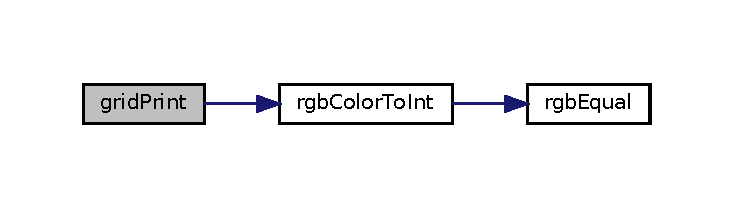
\includegraphics[width=350pt]{grid_8c_ad1e0b52bf8891e9090312f71e9cd5601_cgraph}
\end{center}
\end{figure}
\mbox{\Hypertarget{grid_8c_ab3139f8df42186aa02e725f5bbf2431a}\label{grid_8c_ab3139f8df42186aa02e725f5bbf2431a}} 
\index{grid.\+c@{grid.\+c}!grid\+Print\+Labels@{grid\+Print\+Labels}}
\index{grid\+Print\+Labels@{grid\+Print\+Labels}!grid.\+c@{grid.\+c}}
\subsubsection{\texorpdfstring{grid\+Print\+Labels()}{gridPrintLabels()}}
{\footnotesize\ttfamily grid\+Print\+Labels (\begin{DoxyParamCaption}\item[{\hyperlink{structt__grid}{grid} $\ast$}]{g }\end{DoxyParamCaption})}



Affiche la grille \+: chaque case est représentée par son label. 


\begin{DoxyParams}{Parameters}
{\em g} & \+: la grille \\
\hline
\end{DoxyParams}
Here is the call graph for this function\+:
\nopagebreak
\begin{figure}[H]
\begin{center}
\leavevmode
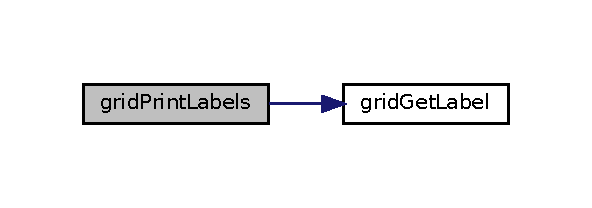
\includegraphics[width=284pt]{grid_8c_ab3139f8df42186aa02e725f5bbf2431a_cgraph}
\end{center}
\end{figure}
\mbox{\Hypertarget{grid_8c_a81c316eaecce336147a01cc72ae90801}\label{grid_8c_a81c316eaecce336147a01cc72ae90801}} 
\index{grid.\+c@{grid.\+c}!grid\+Set\+Color@{grid\+Set\+Color}}
\index{grid\+Set\+Color@{grid\+Set\+Color}!grid.\+c@{grid.\+c}}
\subsubsection{\texorpdfstring{grid\+Set\+Color()}{gridSetColor()}}
{\footnotesize\ttfamily grid\+Set\+Color (\begin{DoxyParamCaption}\item[{\hyperlink{structt__grid}{grid} $\ast$}]{g,  }\item[{\hyperlink{structt___r_g_b}{R\+GB}}]{new\+Color,  }\item[{int}]{x,  }\item[{int}]{y }\end{DoxyParamCaption})}



Affecte une couleur à une case d\textquotesingle{}une grille. 


\begin{DoxyParams}{Parameters}
{\em g} & \+: la grille \\
\hline
{\em new\+Color} & \+: la couleur à affecter en code R\+GB \\
\hline
{\em x} & \+: numéro de la ligne qui contient la case visée \\
\hline
{\em y} & \+: numéro de la colonne qui contient la case visée \\
\hline
\end{DoxyParams}
\mbox{\Hypertarget{grid_8c_a9915684f28fcfbfab54b8cb8cc019057}\label{grid_8c_a9915684f28fcfbfab54b8cb8cc019057}} 
\index{grid.\+c@{grid.\+c}!grid\+Set\+Label@{grid\+Set\+Label}}
\index{grid\+Set\+Label@{grid\+Set\+Label}!grid.\+c@{grid.\+c}}
\subsubsection{\texorpdfstring{grid\+Set\+Label()}{gridSetLabel()}}
{\footnotesize\ttfamily grid\+Set\+Label (\begin{DoxyParamCaption}\item[{\hyperlink{structt__grid}{grid} $\ast$}]{g,  }\item[{int}]{new\+Label,  }\item[{int}]{x,  }\item[{int}]{y }\end{DoxyParamCaption})}



Associe un label à une case de la grille. 


\begin{DoxyParams}{Parameters}
{\em g} & \+: la grille \\
\hline
{\em new\+Label} & \+: le label à associer \\
\hline
{\em x} & \+: numéro de la ligne qui contient la case visée \\
\hline
{\em y} & \+: numéro de la colonne qui contient la case visée \\
\hline
\end{DoxyParams}
\begin{DoxyReturn}{Returns}
Le numéro de la composante connexe de la case. 
\end{DoxyReturn}

\hypertarget{rgb_8c}{}\section{src/game/rgb.c File Reference}
\label{rgb_8c}\index{src/game/rgb.\+c@{src/game/rgb.\+c}}


Gestion des couleurs.  


{\ttfamily \#include \char`\"{}rgb.\+h\char`\"{}}\newline
Include dependency graph for rgb.\+c\+:
\nopagebreak
\begin{figure}[H]
\begin{center}
\leavevmode
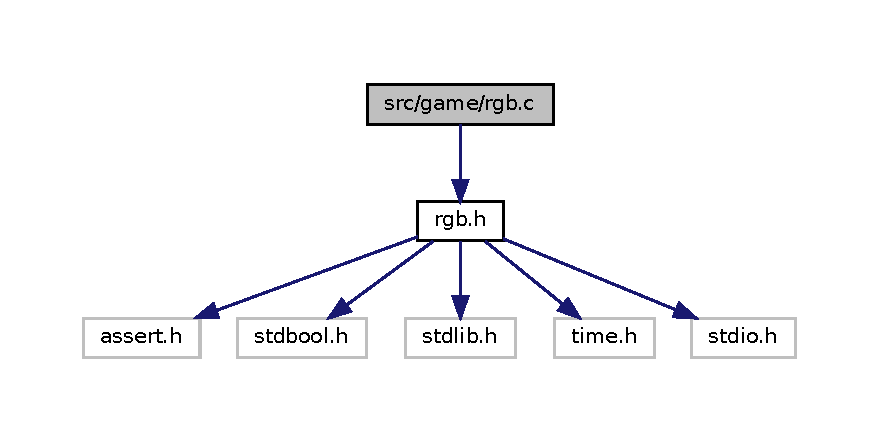
\includegraphics[width=350pt]{rgb_8c__incl}
\end{center}
\end{figure}
\subsection*{Functions}
\begin{DoxyCompactItemize}
\item 
\hyperlink{structt___r_g_b}{R\+GB} \hyperlink{rgb_8c_a7f6b53fea06197bd16137f5da5ea72cf}{rgb\+New} (int R, int G, int B)
\begin{DoxyCompactList}\small\item\em Créer une couleur en utilisant les valeurs données de chaque composante. \end{DoxyCompactList}\item 
\hyperlink{structt___r_g_b}{R\+GB} $\ast$ \hyperlink{rgb_8c_aea93cdd2750c8338054e51f6fdaa4ea0}{rgb\+Import} (F\+I\+LE $\ast$fp, int c\+Nb)
\begin{DoxyCompactList}\small\item\em Importe des couleurs à partir d\textquotesingle{}un fichier. \end{DoxyCompactList}\item 
void \hyperlink{rgb_8c_a670726318c048b47fe78b027bad809d7}{rgb\+Export} (F\+I\+LE $\ast$fp, \hyperlink{structt___r_g_b}{R\+GB} $\ast$c\+Tab, int c\+Nb)
\begin{DoxyCompactList}\small\item\em Exporte un tableau de couleurs dans un fichier. \end{DoxyCompactList}\item 
void \hyperlink{rgb_8c_a7df3eec610b0fa98a5ccb1cf6a9b00ef}{rgb\+Print} (\hyperlink{structt___r_g_b}{R\+GB} c)
\begin{DoxyCompactList}\small\item\em Affiche les trois composantes de la couleur dans la console. \end{DoxyCompactList}\item 
void \hyperlink{rgb_8c_af5947037ec0678e4bafc967877cfbb35}{rgb\+Array\+Print} (\hyperlink{structt___r_g_b}{R\+GB} $\ast$tab, int size)
\begin{DoxyCompactList}\small\item\em Affiche un tableau contenant plusieurs couleurs dans la console. \end{DoxyCompactList}\item 
\hyperlink{structt___r_g_b}{R\+GB} \hyperlink{rgb_8c_a0fe7dfd1dca25f3443104c9135510f17}{rgb\+Gen\+Rand} ()
\begin{DoxyCompactList}\small\item\em Genère une couleur au hasard. \end{DoxyCompactList}\item 
\hyperlink{structt___r_g_b}{R\+GB} $\ast$ \hyperlink{rgb_8c_a195f303207c06d72f092e34d20b6ef25}{rgb\+Array\+Gen\+Rand} (int nb)
\begin{DoxyCompactList}\small\item\em Génère un tableau de couleurs au hasard. \end{DoxyCompactList}\item 
bool \hyperlink{rgb_8c_a42e73f2513cb6a6fc188fc2c60eed9c9}{rgb\+Array\+Has\+Duplicate} (\hyperlink{structt___r_g_b}{R\+GB} $\ast$tab, int size)
\begin{DoxyCompactList}\small\item\em Teste une tableau de couleurs pour savoir si deux couleurs sont les mêmes. \end{DoxyCompactList}\item 
bool \hyperlink{rgb_8c_a69f8efffc6c16e0b2379dbc3467d5364}{rgb\+Equal} (\hyperlink{structt___r_g_b}{R\+GB} c1, \hyperlink{structt___r_g_b}{R\+GB} c2)
\begin{DoxyCompactList}\small\item\em Teste deux couleurs pour savoir si ce sont les mêmes. \end{DoxyCompactList}\item 
int \hyperlink{rgb_8c_adafe178d2850e09e825de82e12f5c293}{rgb\+Color\+To\+Int} (\hyperlink{structt___r_g_b}{R\+GB} c, \hyperlink{structt___r_g_b}{R\+GB} $\ast$tab, int size)
\begin{DoxyCompactList}\small\item\em Cherche une couleur donnée dans un tableau de couleurs. \end{DoxyCompactList}\item 
void \hyperlink{rgb_8c_a7310155c8ae06c73cfeff47165077e68}{rgb\+Array\+Free} (\hyperlink{structt___r_g_b}{R\+GB} $\ast$tab)
\begin{DoxyCompactList}\small\item\em Supprime un tableau de couleurs. \end{DoxyCompactList}\end{DoxyCompactItemize}


\subsection{Detailed Description}
Gestion des couleurs. 

\begin{DoxyAuthor}{Author}
Last\+But\+Not\+Least 
\end{DoxyAuthor}
\begin{DoxyDate}{Date}
Mars 2017 
\end{DoxyDate}


\subsection{Function Documentation}
\mbox{\Hypertarget{rgb_8c_a7310155c8ae06c73cfeff47165077e68}\label{rgb_8c_a7310155c8ae06c73cfeff47165077e68}} 
\index{rgb.\+c@{rgb.\+c}!rgb\+Array\+Free@{rgb\+Array\+Free}}
\index{rgb\+Array\+Free@{rgb\+Array\+Free}!rgb.\+c@{rgb.\+c}}
\subsubsection{\texorpdfstring{rgb\+Array\+Free()}{rgbArrayFree()}}
{\footnotesize\ttfamily rgb\+Array\+Free (\begin{DoxyParamCaption}\item[{\hyperlink{structt___r_g_b}{R\+GB} $\ast$}]{tab }\end{DoxyParamCaption})}



Supprime un tableau de couleurs. 


\begin{DoxyParams}{Parameters}
{\em tab} & \+: le tableau à supprimer \\
\hline
\end{DoxyParams}
\mbox{\Hypertarget{rgb_8c_a195f303207c06d72f092e34d20b6ef25}\label{rgb_8c_a195f303207c06d72f092e34d20b6ef25}} 
\index{rgb.\+c@{rgb.\+c}!rgb\+Array\+Gen\+Rand@{rgb\+Array\+Gen\+Rand}}
\index{rgb\+Array\+Gen\+Rand@{rgb\+Array\+Gen\+Rand}!rgb.\+c@{rgb.\+c}}
\subsubsection{\texorpdfstring{rgb\+Array\+Gen\+Rand()}{rgbArrayGenRand()}}
{\footnotesize\ttfamily rgb\+Array\+Gen\+Rand (\begin{DoxyParamCaption}\item[{int}]{nb }\end{DoxyParamCaption})}



Génère un tableau de couleurs au hasard. 

\+: la taille du tableau doit être non nulle. 
\begin{DoxyParams}{Parameters}
{\em nb} & \+: taille du tableau à générer. \\
\hline
\end{DoxyParams}
\begin{DoxyReturn}{Returns}
Le tableau de couleurs avec le code R\+GB. 
\end{DoxyReturn}
Here is the call graph for this function\+:
\nopagebreak
\begin{figure}[H]
\begin{center}
\leavevmode
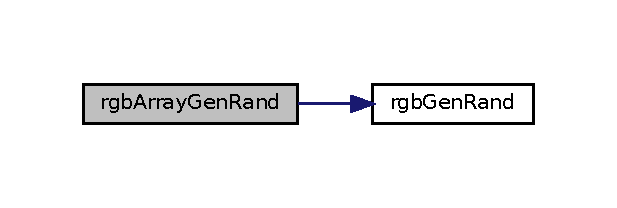
\includegraphics[width=296pt]{rgb_8c_a195f303207c06d72f092e34d20b6ef25_cgraph}
\end{center}
\end{figure}
\mbox{\Hypertarget{rgb_8c_a42e73f2513cb6a6fc188fc2c60eed9c9}\label{rgb_8c_a42e73f2513cb6a6fc188fc2c60eed9c9}} 
\index{rgb.\+c@{rgb.\+c}!rgb\+Array\+Has\+Duplicate@{rgb\+Array\+Has\+Duplicate}}
\index{rgb\+Array\+Has\+Duplicate@{rgb\+Array\+Has\+Duplicate}!rgb.\+c@{rgb.\+c}}
\subsubsection{\texorpdfstring{rgb\+Array\+Has\+Duplicate()}{rgbArrayHasDuplicate()}}
{\footnotesize\ttfamily rgb\+Array\+Has\+Duplicate (\begin{DoxyParamCaption}\item[{\hyperlink{structt___r_g_b}{R\+GB} $\ast$}]{tab,  }\item[{int}]{size }\end{DoxyParamCaption})}



Teste une tableau de couleurs pour savoir si deux couleurs sont les mêmes. 


\begin{DoxyParams}{Parameters}
{\em tab} & \+: le tableau de couleurs \\
\hline
{\em size} & \+: la taille du tableau \\
\hline
\end{DoxyParams}
\begin{DoxyReturn}{Returns}
true s\textquotesingle{}il y a deux couleurs identiques, false sinon. 
\end{DoxyReturn}
Here is the call graph for this function\+:
\nopagebreak
\begin{figure}[H]
\begin{center}
\leavevmode
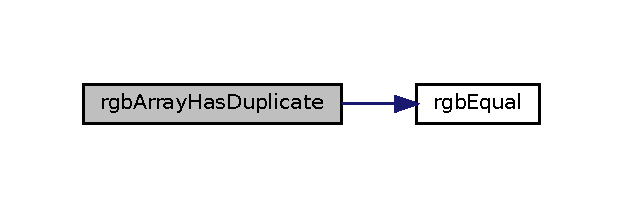
\includegraphics[width=299pt]{rgb_8c_a42e73f2513cb6a6fc188fc2c60eed9c9_cgraph}
\end{center}
\end{figure}
\mbox{\Hypertarget{rgb_8c_af5947037ec0678e4bafc967877cfbb35}\label{rgb_8c_af5947037ec0678e4bafc967877cfbb35}} 
\index{rgb.\+c@{rgb.\+c}!rgb\+Array\+Print@{rgb\+Array\+Print}}
\index{rgb\+Array\+Print@{rgb\+Array\+Print}!rgb.\+c@{rgb.\+c}}
\subsubsection{\texorpdfstring{rgb\+Array\+Print()}{rgbArrayPrint()}}
{\footnotesize\ttfamily rgb\+Array\+Print (\begin{DoxyParamCaption}\item[{\hyperlink{structt___r_g_b}{R\+GB} $\ast$}]{tab,  }\item[{int}]{size }\end{DoxyParamCaption})}



Affiche un tableau contenant plusieurs couleurs dans la console. 


\begin{DoxyParams}{Parameters}
{\em tab} & \+: le tableau qui contient les couleurs \\
\hline
{\em size} & \+: nombre de couleurs dans le tableau \\
\hline
\end{DoxyParams}
Here is the call graph for this function\+:
\nopagebreak
\begin{figure}[H]
\begin{center}
\leavevmode
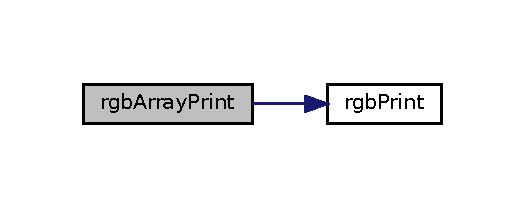
\includegraphics[width=252pt]{rgb_8c_af5947037ec0678e4bafc967877cfbb35_cgraph}
\end{center}
\end{figure}
\mbox{\Hypertarget{rgb_8c_adafe178d2850e09e825de82e12f5c293}\label{rgb_8c_adafe178d2850e09e825de82e12f5c293}} 
\index{rgb.\+c@{rgb.\+c}!rgb\+Color\+To\+Int@{rgb\+Color\+To\+Int}}
\index{rgb\+Color\+To\+Int@{rgb\+Color\+To\+Int}!rgb.\+c@{rgb.\+c}}
\subsubsection{\texorpdfstring{rgb\+Color\+To\+Int()}{rgbColorToInt()}}
{\footnotesize\ttfamily rgb\+Color\+To\+Int (\begin{DoxyParamCaption}\item[{\hyperlink{structt___r_g_b}{R\+GB}}]{c,  }\item[{\hyperlink{structt___r_g_b}{R\+GB} $\ast$}]{tab,  }\item[{int}]{size }\end{DoxyParamCaption})}



Cherche une couleur donnée dans un tableau de couleurs. 


\begin{DoxyParams}{Parameters}
{\em c} & \+: la couleur cherchée \\
\hline
{\em tab} & \+: le tableau de couleurs \\
\hline
{\em size} & \+: la taille du tableau \\
\hline
\end{DoxyParams}
\begin{DoxyReturn}{Returns}
Le rang de la couleur dans le tableau si elle a été trouvée ; -\/1 sinon. 
\end{DoxyReturn}
Here is the call graph for this function\+:
\nopagebreak
\begin{figure}[H]
\begin{center}
\leavevmode
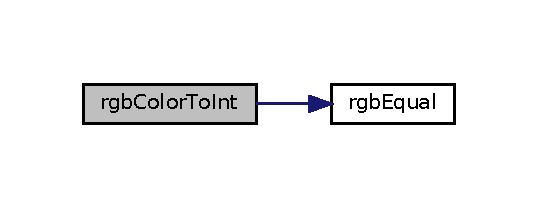
\includegraphics[width=258pt]{rgb_8c_adafe178d2850e09e825de82e12f5c293_cgraph}
\end{center}
\end{figure}
\mbox{\Hypertarget{rgb_8c_a69f8efffc6c16e0b2379dbc3467d5364}\label{rgb_8c_a69f8efffc6c16e0b2379dbc3467d5364}} 
\index{rgb.\+c@{rgb.\+c}!rgb\+Equal@{rgb\+Equal}}
\index{rgb\+Equal@{rgb\+Equal}!rgb.\+c@{rgb.\+c}}
\subsubsection{\texorpdfstring{rgb\+Equal()}{rgbEqual()}}
{\footnotesize\ttfamily rgb\+Equal (\begin{DoxyParamCaption}\item[{\hyperlink{structt___r_g_b}{R\+GB}}]{c1,  }\item[{\hyperlink{structt___r_g_b}{R\+GB}}]{c2 }\end{DoxyParamCaption})}



Teste deux couleurs pour savoir si ce sont les mêmes. 


\begin{DoxyParams}{Parameters}
{\em c1} & \+: la première couleur \\
\hline
{\em c2} & \+: la deuxième couleur \\
\hline
\end{DoxyParams}
\begin{DoxyReturn}{Returns}
true si les couleurs sont les mêmes, false sinon. 
\end{DoxyReturn}
\mbox{\Hypertarget{rgb_8c_a670726318c048b47fe78b027bad809d7}\label{rgb_8c_a670726318c048b47fe78b027bad809d7}} 
\index{rgb.\+c@{rgb.\+c}!rgb\+Export@{rgb\+Export}}
\index{rgb\+Export@{rgb\+Export}!rgb.\+c@{rgb.\+c}}
\subsubsection{\texorpdfstring{rgb\+Export()}{rgbExport()}}
{\footnotesize\ttfamily rgb\+Export (\begin{DoxyParamCaption}\item[{F\+I\+LE $\ast$}]{fp,  }\item[{\hyperlink{structt___r_g_b}{R\+GB} $\ast$}]{c\+Tab,  }\item[{int}]{c\+Nb }\end{DoxyParamCaption})}



Exporte un tableau de couleurs dans un fichier. 


\begin{DoxyParams}{Parameters}
{\em fp} & \+: le fichier \\
\hline
{\em c\+Tab} & \+: le tableau de couleurs \\
\hline
{\em c\+Nb} & \+: le nombre de couleurs différentes \\
\hline
\end{DoxyParams}
\mbox{\Hypertarget{rgb_8c_a0fe7dfd1dca25f3443104c9135510f17}\label{rgb_8c_a0fe7dfd1dca25f3443104c9135510f17}} 
\index{rgb.\+c@{rgb.\+c}!rgb\+Gen\+Rand@{rgb\+Gen\+Rand}}
\index{rgb\+Gen\+Rand@{rgb\+Gen\+Rand}!rgb.\+c@{rgb.\+c}}
\subsubsection{\texorpdfstring{rgb\+Gen\+Rand()}{rgbGenRand()}}
{\footnotesize\ttfamily rgb\+Gen\+Rand (\begin{DoxyParamCaption}{ }\end{DoxyParamCaption})}



Genère une couleur au hasard. 

\begin{DoxyReturn}{Returns}
La couleur générée avec le code R\+GB. 
\end{DoxyReturn}
\mbox{\Hypertarget{rgb_8c_aea93cdd2750c8338054e51f6fdaa4ea0}\label{rgb_8c_aea93cdd2750c8338054e51f6fdaa4ea0}} 
\index{rgb.\+c@{rgb.\+c}!rgb\+Import@{rgb\+Import}}
\index{rgb\+Import@{rgb\+Import}!rgb.\+c@{rgb.\+c}}
\subsubsection{\texorpdfstring{rgb\+Import()}{rgbImport()}}
{\footnotesize\ttfamily rgb\+Import (\begin{DoxyParamCaption}\item[{F\+I\+LE $\ast$}]{fp,  }\item[{int}]{c\+Nb }\end{DoxyParamCaption})}



Importe des couleurs à partir d\textquotesingle{}un fichier. 


\begin{DoxyParams}{Parameters}
{\em fp} & \+: le fichier \\
\hline
{\em c\+Nb} & \+: nombre de couleurs différentes \\
\hline
\end{DoxyParams}
\begin{DoxyReturn}{Returns}
un tableau contenant les couleurs importées 
\end{DoxyReturn}
Here is the call graph for this function\+:
\nopagebreak
\begin{figure}[H]
\begin{center}
\leavevmode
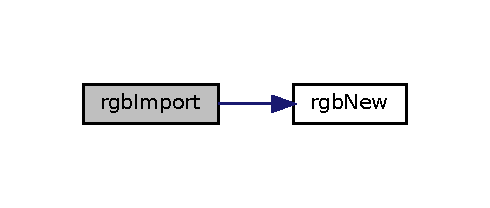
\includegraphics[width=235pt]{rgb_8c_aea93cdd2750c8338054e51f6fdaa4ea0_cgraph}
\end{center}
\end{figure}
\mbox{\Hypertarget{rgb_8c_a7f6b53fea06197bd16137f5da5ea72cf}\label{rgb_8c_a7f6b53fea06197bd16137f5da5ea72cf}} 
\index{rgb.\+c@{rgb.\+c}!rgb\+New@{rgb\+New}}
\index{rgb\+New@{rgb\+New}!rgb.\+c@{rgb.\+c}}
\subsubsection{\texorpdfstring{rgb\+New()}{rgbNew()}}
{\footnotesize\ttfamily rgb\+New (\begin{DoxyParamCaption}\item[{int}]{R,  }\item[{int}]{G,  }\item[{int}]{B }\end{DoxyParamCaption})}



Créer une couleur en utilisant les valeurs données de chaque composante. 


\begin{DoxyParams}{Parameters}
{\em R} & \+: composante rouge (max 256) \\
\hline
{\em G} & \+: composante verte (max 256) \\
\hline
{\em B} & \+: composante bleue (max 256) \\
\hline
\end{DoxyParams}
\begin{DoxyReturn}{Returns}
\+: la couleur (en code R\+GB) 
\end{DoxyReturn}
\mbox{\Hypertarget{rgb_8c_a7df3eec610b0fa98a5ccb1cf6a9b00ef}\label{rgb_8c_a7df3eec610b0fa98a5ccb1cf6a9b00ef}} 
\index{rgb.\+c@{rgb.\+c}!rgb\+Print@{rgb\+Print}}
\index{rgb\+Print@{rgb\+Print}!rgb.\+c@{rgb.\+c}}
\subsubsection{\texorpdfstring{rgb\+Print()}{rgbPrint()}}
{\footnotesize\ttfamily rgb\+Print (\begin{DoxyParamCaption}\item[{\hyperlink{structt___r_g_b}{R\+GB}}]{c }\end{DoxyParamCaption})}



Affiche les trois composantes de la couleur dans la console. 


\begin{DoxyParams}{Parameters}
{\em c} & \+: une couleur \\
\hline
\end{DoxyParams}

\hypertarget{solver_8c}{}\section{src/solver/solver.c File Reference}
\label{solver_8c}\index{src/solver/solver.\+c@{src/solver/solver.\+c}}


Gestion du solveur.  


{\ttfamily \#include \char`\"{}solver.\+h\char`\"{}}\newline
Include dependency graph for solver.\+c\+:
\nopagebreak
\begin{figure}[H]
\begin{center}
\leavevmode
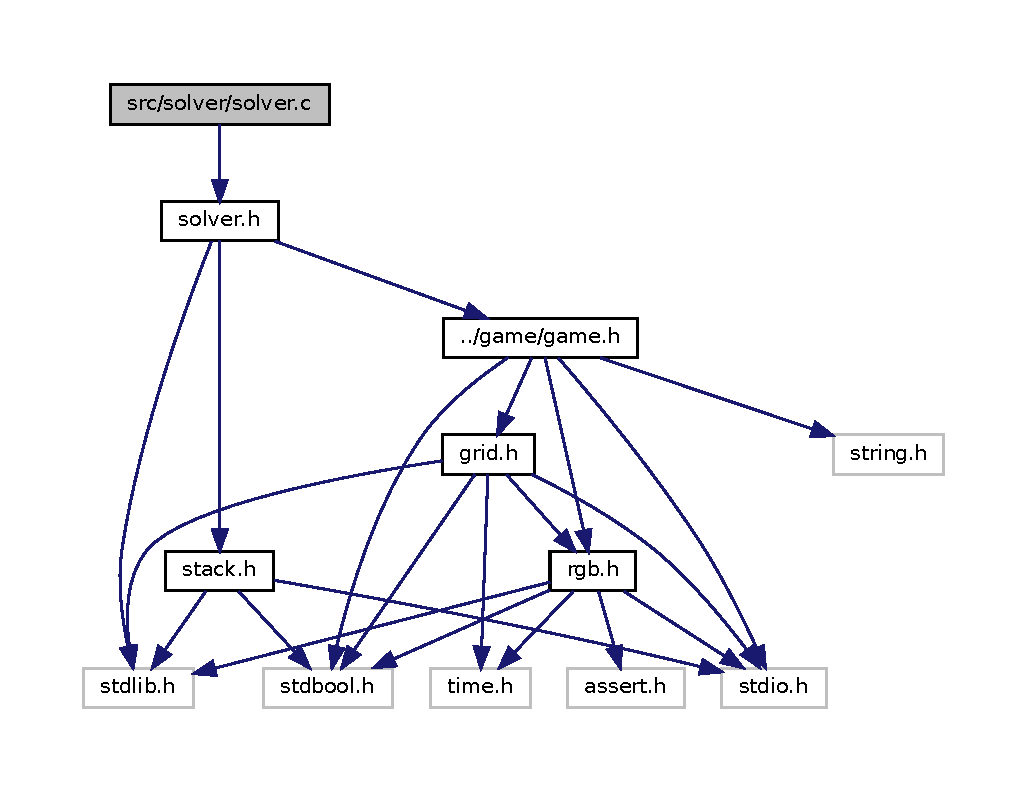
\includegraphics[width=350pt]{solver_8c__incl}
\end{center}
\end{figure}
\subsection*{Functions}
\begin{DoxyCompactItemize}
\item 
int \hyperlink{solver_8c_ae5efa588412134b93ddda2061176d8be}{print\+Best} (\hyperlink{structt__game}{game} $\ast$g)
\begin{DoxyCompactList}\small\item\em Trouve une solution par bruteforce si taille $<$ 9, par heuristique sinon, l\textquotesingle{}affiche dans la console, et retourne sa taille. \end{DoxyCompactList}\item 
void \hyperlink{solver_8c_ac5c6b2c33d2447269800806135e1d829}{process\+Neighbours} (\hyperlink{structt__game}{game} $\ast$g, int x, int y, int $\ast$adj\+Matrix)
\begin{DoxyCompactList}\small\item\em Modifie la matrice d\textquotesingle{}adjacence. \end{DoxyCompactList}\item 
int $\ast$ \hyperlink{solver_8c_a61c82bfe85ab52391aff217dc4afc75c}{solver\+Compute\+Adj\+Matrix} (\hyperlink{structt__game}{game} $\ast$g)
\begin{DoxyCompactList}\small\item\em Crée la matrice d\textquotesingle{}adjacence associée à une partie. \end{DoxyCompactList}\item 
int $\ast$ \hyperlink{solver_8c_a958c071239440919668cf9df4f7fff13}{solver\+Compute\+Lbl\+To\+Color\+Array} (\hyperlink{structt__game}{game} $\ast$g)
\begin{DoxyCompactList}\small\item\em Crée un tableau qui contient en i-\/ème position la couleur du i-\/ème label. \end{DoxyCompactList}\item 
bool \hyperlink{solver_8c_aaf2dd01fab598cfd3e1fc92ab727da35}{solver\+Game\+Over} (const int $\ast$player\+Labels, const int max\+Label)
\begin{DoxyCompactList}\small\item\em Teste si la partie est finie. \end{DoxyCompactList}\item 
void \hyperlink{solver_8c_acf0c40dd323ca07d656f475f672681f9}{solve\+Brute\+Force} (const int $\ast$adj\+Matrix, const int $\ast$lbl\+To\+Color, int $\ast$player\+Labels, const int max\+Label, const int color\+Range, int $\ast$max\+Depth, int curr\+Depth, \hyperlink{structnode}{stack} solution, \hyperlink{structnode}{stack} $\ast$best, int played\+Color)
\begin{DoxyCompactList}\small\item\em Retourne dans la stack best la meilleure solution. \end{DoxyCompactList}\item 
void \hyperlink{solver_8c_ad0d28f9e5b065430ab0cc7cb51c91c8d}{solve\+Heuristic} (const int $\ast$adj\+Matrix, const int $\ast$lbl\+To\+Color, int $\ast$player\+Labels, const int max\+Label, const int color\+Range, int $\ast$max\+Depth, int curr\+Depth, \hyperlink{structnode}{stack} solution, \hyperlink{structnode}{stack} $\ast$best, int played\+Color)
\begin{DoxyCompactList}\small\item\em Retourne dans la stack best la solution trouvée en coloriant le maximum de composantes connexes a chaque tour (NB\+: Copier/\+Coller modifié de la fonction solve\+Brute\+Force, une seule stack suffirait) \end{DoxyCompactList}\end{DoxyCompactItemize}


\subsection{Detailed Description}
Gestion du solveur. 

\begin{DoxyAuthor}{Author}
Last\+But\+Not\+Least 
\end{DoxyAuthor}
\begin{DoxyDate}{Date}
Mai 2017 
\end{DoxyDate}


\subsection{Function Documentation}
\mbox{\Hypertarget{solver_8c_ae5efa588412134b93ddda2061176d8be}\label{solver_8c_ae5efa588412134b93ddda2061176d8be}} 
\index{solver.\+c@{solver.\+c}!print\+Best@{print\+Best}}
\index{print\+Best@{print\+Best}!solver.\+c@{solver.\+c}}
\subsubsection{\texorpdfstring{print\+Best()}{printBest()}}
{\footnotesize\ttfamily print\+Best (\begin{DoxyParamCaption}\item[{\hyperlink{structt__game}{game} $\ast$}]{g }\end{DoxyParamCaption})}



Trouve une solution par bruteforce si taille $<$ 9, par heuristique sinon, l\textquotesingle{}affiche dans la console, et retourne sa taille. 


\begin{DoxyParams}{Parameters}
{\em g} & \+: la partie \\
\hline
\end{DoxyParams}
\begin{DoxyReturn}{Returns}
la taille de la solution 
\end{DoxyReturn}
Here is the call graph for this function\+:
\nopagebreak
\begin{figure}[H]
\begin{center}
\leavevmode
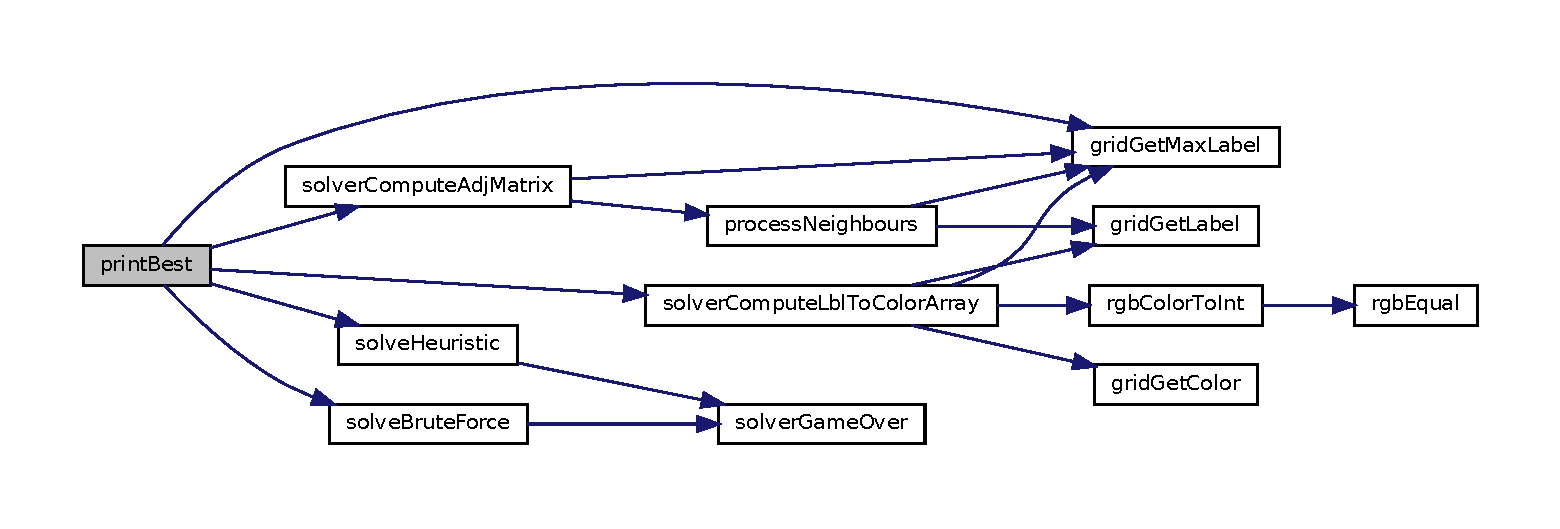
\includegraphics[width=350pt]{solver_8c_ae5efa588412134b93ddda2061176d8be_cgraph}
\end{center}
\end{figure}
\mbox{\Hypertarget{solver_8c_ac5c6b2c33d2447269800806135e1d829}\label{solver_8c_ac5c6b2c33d2447269800806135e1d829}} 
\index{solver.\+c@{solver.\+c}!process\+Neighbours@{process\+Neighbours}}
\index{process\+Neighbours@{process\+Neighbours}!solver.\+c@{solver.\+c}}
\subsubsection{\texorpdfstring{process\+Neighbours()}{processNeighbours()}}
{\footnotesize\ttfamily process\+Neighbours (\begin{DoxyParamCaption}\item[{\hyperlink{structt__game}{game} $\ast$}]{g,  }\item[{int}]{x,  }\item[{int}]{y,  }\item[{int $\ast$}]{adj\+Matrix }\end{DoxyParamCaption})}



Modifie la matrice d\textquotesingle{}adjacence. 

On choisit une case de la grille, on obtient son label et le label d\textquotesingle{}une case voisine \+: ces deux nombres sont les coordonnées dans la matrice d\textquotesingle{}une case où on inscrit 1. On procède de même pour chaque case voisine.

Les autres cases sont laissées à 0.


\begin{DoxyParams}{Parameters}
{\em g} & \+: la partie \\
\hline
{\em x} & \+: ligne de la case choisie \\
\hline
{\em y} & \+: colonne de la case choisie \\
\hline
{\em adj\+Matrix} & \+: la matrice d\textquotesingle{}adjacence à modifier \\
\hline
\end{DoxyParams}
\begin{DoxyReturn}{Returns}
La matriche d\textquotesingle{}adjacence modifiée 
\end{DoxyReturn}
Here is the call graph for this function\+:
\nopagebreak
\begin{figure}[H]
\begin{center}
\leavevmode
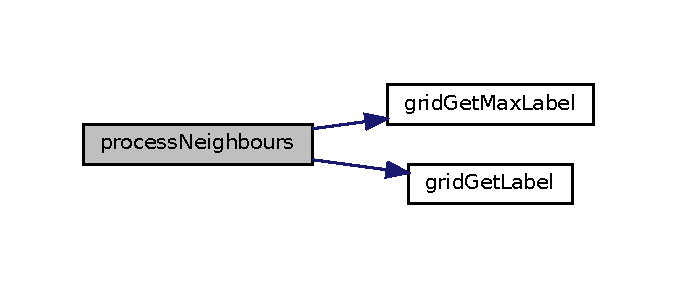
\includegraphics[width=325pt]{solver_8c_ac5c6b2c33d2447269800806135e1d829_cgraph}
\end{center}
\end{figure}
\mbox{\Hypertarget{solver_8c_acf0c40dd323ca07d656f475f672681f9}\label{solver_8c_acf0c40dd323ca07d656f475f672681f9}} 
\index{solver.\+c@{solver.\+c}!solve\+Brute\+Force@{solve\+Brute\+Force}}
\index{solve\+Brute\+Force@{solve\+Brute\+Force}!solver.\+c@{solver.\+c}}
\subsubsection{\texorpdfstring{solve\+Brute\+Force()}{solveBruteForce()}}
{\footnotesize\ttfamily solve\+Brute\+Force (\begin{DoxyParamCaption}\item[{const int $\ast$}]{adj\+Matrix,  }\item[{const int $\ast$}]{lbl\+To\+Color,  }\item[{int $\ast$}]{player\+Labels,  }\item[{const int}]{max\+Label,  }\item[{const int}]{color\+Range,  }\item[{int $\ast$}]{max\+Depth,  }\item[{int}]{curr\+Depth,  }\item[{\hyperlink{structnode}{stack}}]{solution,  }\item[{\hyperlink{structnode}{stack} $\ast$}]{best,  }\item[{int}]{played\+Color }\end{DoxyParamCaption})}



Retourne dans la stack best la meilleure solution. 


\begin{DoxyParams}{Parameters}
{\em adj\+Matrix} & \+: la matrice d\textquotesingle{}adjacence \\
\hline
{\em lbl\+To\+Color} & \+: la tableau qui associe à chaque label sa souleur \\
\hline
{\em player\+Labels} & \+: tableau qui contient en i-\/ème position 1 si le i-\/ème label a déjà été connecté au label actuel, 0 sinon \\
\hline
{\em max\+Label} & \+: label maximal \\
\hline
{\em color\+Range} & \+: nombre de couleurs \\
\hline
{\em max\+Depth} & \+: nombre de coups joués dans la meilleure solution \\
\hline
{\em curr\+Depth} & \+: nombre de coups dans la solution actuelle \\
\hline
{\em solution} & \+: la solution actuelle \\
\hline
{\em best} & \+: la meilleure solution \\
\hline
{\em played\+Color} & \+: la couleur à jouer \\
\hline
\end{DoxyParams}
Here is the call graph for this function\+:
\nopagebreak
\begin{figure}[H]
\begin{center}
\leavevmode
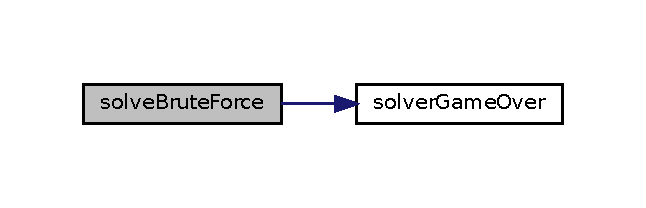
\includegraphics[width=310pt]{solver_8c_acf0c40dd323ca07d656f475f672681f9_cgraph}
\end{center}
\end{figure}
\mbox{\Hypertarget{solver_8c_ad0d28f9e5b065430ab0cc7cb51c91c8d}\label{solver_8c_ad0d28f9e5b065430ab0cc7cb51c91c8d}} 
\index{solver.\+c@{solver.\+c}!solve\+Heuristic@{solve\+Heuristic}}
\index{solve\+Heuristic@{solve\+Heuristic}!solver.\+c@{solver.\+c}}
\subsubsection{\texorpdfstring{solve\+Heuristic()}{solveHeuristic()}}
{\footnotesize\ttfamily solve\+Heuristic (\begin{DoxyParamCaption}\item[{const int $\ast$}]{adj\+Matrix,  }\item[{const int $\ast$}]{lbl\+To\+Color,  }\item[{int $\ast$}]{player\+Labels,  }\item[{const int}]{max\+Label,  }\item[{const int}]{color\+Range,  }\item[{int $\ast$}]{max\+Depth,  }\item[{int}]{curr\+Depth,  }\item[{\hyperlink{structnode}{stack}}]{solution,  }\item[{\hyperlink{structnode}{stack} $\ast$}]{best,  }\item[{int}]{played\+Color }\end{DoxyParamCaption})}



Retourne dans la stack best la solution trouvée en coloriant le maximum de composantes connexes a chaque tour (NB\+: Copier/\+Coller modifié de la fonction solve\+Brute\+Force, une seule stack suffirait) 


\begin{DoxyParams}{Parameters}
{\em adj\+Matrix} & \+: la matrice d\textquotesingle{}adjacence \\
\hline
{\em lbl\+To\+Color} & \+: la tableau qui associe à chaque label sa souleur \\
\hline
{\em player\+Labels} & \+: tableau qui contient en i-\/ème position 1 si le i-\/ème label a déjà été connecté au label actuel, 0 sinon \\
\hline
{\em max\+Label} & \+: label maximal \\
\hline
{\em color\+Range} & \+: nombre de couleurs \\
\hline
{\em max\+Depth} & \+: nombre de coups joués dans la meilleure solution \\
\hline
{\em curr\+Depth} & \+: nombre de coups dans la solution actuelle \\
\hline
{\em solution} & \+: la solution actuelle \\
\hline
{\em best} & \+: la meilleure solution \\
\hline
{\em played\+Color} & \+: la couleur à jouer \\
\hline
\end{DoxyParams}
Here is the call graph for this function\+:
\nopagebreak
\begin{figure}[H]
\begin{center}
\leavevmode
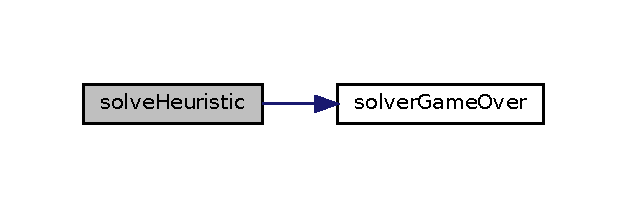
\includegraphics[width=301pt]{solver_8c_ad0d28f9e5b065430ab0cc7cb51c91c8d_cgraph}
\end{center}
\end{figure}
\mbox{\Hypertarget{solver_8c_a61c82bfe85ab52391aff217dc4afc75c}\label{solver_8c_a61c82bfe85ab52391aff217dc4afc75c}} 
\index{solver.\+c@{solver.\+c}!solver\+Compute\+Adj\+Matrix@{solver\+Compute\+Adj\+Matrix}}
\index{solver\+Compute\+Adj\+Matrix@{solver\+Compute\+Adj\+Matrix}!solver.\+c@{solver.\+c}}
\subsubsection{\texorpdfstring{solver\+Compute\+Adj\+Matrix()}{solverComputeAdjMatrix()}}
{\footnotesize\ttfamily solver\+Compute\+Adj\+Matrix (\begin{DoxyParamCaption}\item[{\hyperlink{structt__game}{game} $\ast$}]{g }\end{DoxyParamCaption})}



Crée la matrice d\textquotesingle{}adjacence associée à une partie. 


\begin{DoxyParams}{Parameters}
{\em g} & \+: la partie \\
\hline
\end{DoxyParams}
\begin{DoxyReturn}{Returns}
la matrice d\textquotesingle{}adjacence 
\end{DoxyReturn}
Here is the call graph for this function\+:
\nopagebreak
\begin{figure}[H]
\begin{center}
\leavevmode
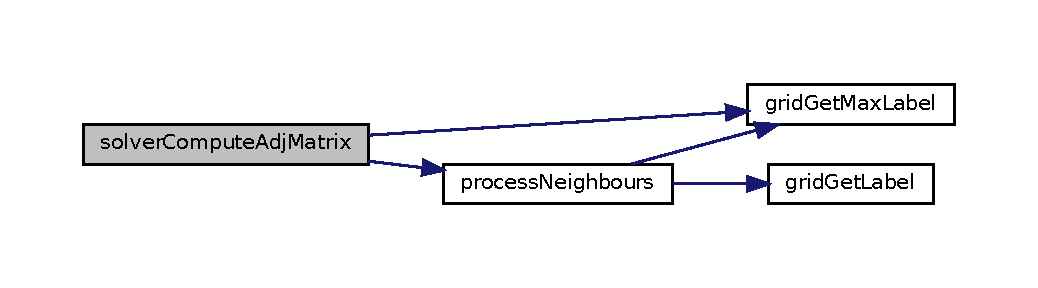
\includegraphics[width=350pt]{solver_8c_a61c82bfe85ab52391aff217dc4afc75c_cgraph}
\end{center}
\end{figure}
\mbox{\Hypertarget{solver_8c_a958c071239440919668cf9df4f7fff13}\label{solver_8c_a958c071239440919668cf9df4f7fff13}} 
\index{solver.\+c@{solver.\+c}!solver\+Compute\+Lbl\+To\+Color\+Array@{solver\+Compute\+Lbl\+To\+Color\+Array}}
\index{solver\+Compute\+Lbl\+To\+Color\+Array@{solver\+Compute\+Lbl\+To\+Color\+Array}!solver.\+c@{solver.\+c}}
\subsubsection{\texorpdfstring{solver\+Compute\+Lbl\+To\+Color\+Array()}{solverComputeLblToColorArray()}}
{\footnotesize\ttfamily solver\+Compute\+Lbl\+To\+Color\+Array (\begin{DoxyParamCaption}\item[{\hyperlink{structt__game}{game} $\ast$}]{g }\end{DoxyParamCaption})}



Crée un tableau qui contient en i-\/ème position la couleur du i-\/ème label. 


\begin{DoxyParams}{Parameters}
{\em g} & \+: la partie \\
\hline
\end{DoxyParams}
\begin{DoxyReturn}{Returns}
le tableau 
\end{DoxyReturn}
Here is the call graph for this function\+:
\nopagebreak
\begin{figure}[H]
\begin{center}
\leavevmode
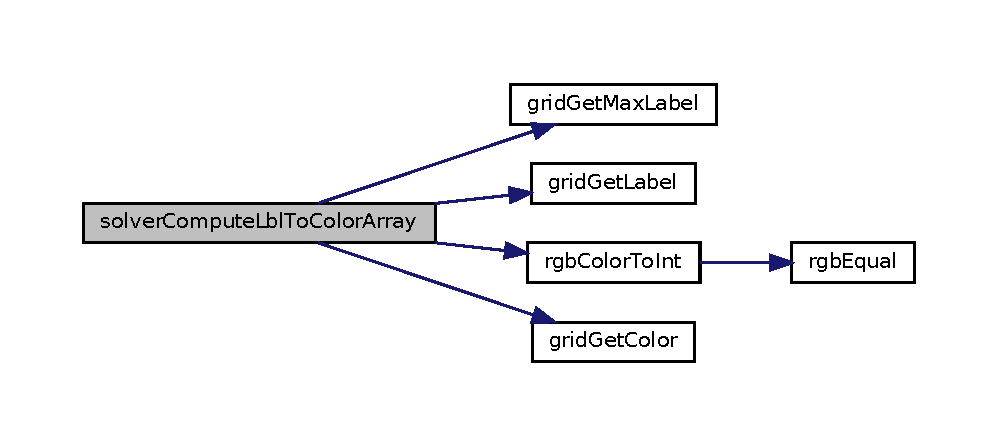
\includegraphics[width=350pt]{solver_8c_a958c071239440919668cf9df4f7fff13_cgraph}
\end{center}
\end{figure}
\mbox{\Hypertarget{solver_8c_aaf2dd01fab598cfd3e1fc92ab727da35}\label{solver_8c_aaf2dd01fab598cfd3e1fc92ab727da35}} 
\index{solver.\+c@{solver.\+c}!solver\+Game\+Over@{solver\+Game\+Over}}
\index{solver\+Game\+Over@{solver\+Game\+Over}!solver.\+c@{solver.\+c}}
\subsubsection{\texorpdfstring{solver\+Game\+Over()}{solverGameOver()}}
{\footnotesize\ttfamily solver\+Game\+Over (\begin{DoxyParamCaption}\item[{const int $\ast$}]{player\+Labels,  }\item[{const int}]{max\+Label }\end{DoxyParamCaption})}



Teste si la partie est finie. 


\begin{DoxyParams}{Parameters}
{\em g} & \+: la partie \\
\hline
\end{DoxyParams}
\begin{DoxyReturn}{Returns}
true si la partie est finie, false sinon 
\end{DoxyReturn}

%--- End generated contents ---

% Index
\backmatter
\newpage
\phantomsection
\clearemptydoublepage
\addcontentsline{toc}{chapter}{Index}
\printindex

\end{document}
